% !TEX TS-program = pdflatex
% Main report — Autonomous TEC-Based PV Cleaning Robot
% Multi-scale design for Egyptian new cities
% Run: python scripts/project_calculations.py before first compile.
\documentclass[12pt,a4paper]{report}   % REE 598 format: 12 pt base

\usepackage[margin=2.5cm]{geometry}
\usepackage[T1]{fontenc}
\usepackage{amsmath,amssymb}
\usepackage{mathptmx}                   % Times New Roman compatible text + math (REE 598 format)
\usepackage{microtype}
\setlength{\emergencystretch}{3em}       % absorb long \texttt{} paths so they don't overflow the margin
\usepackage{setspace}
\onehalfspacing                         % 1.5 line spacing (REE 598 format)
\usepackage{booktabs}
\usepackage{array}
\usepackage{tabularx}
\usepackage{multirow}
\usepackage{enumitem}
\usepackage{graphicx}
\usepackage{fancyvrb}
\usepackage{xcolor}                     % colour for the Gantt chart (rule-bar style)
\usepackage{siunitx}                    % SI units (REE 598/599 format)
\sisetup{group-separator={,},group-minimum-digits=4}
\usepackage{caption}
\usepackage{pdflscape}
\usepackage[hidelinks]{hyperref}
\usepackage{xurl}
\makeatletter
\g@addto@macro{\UrlBreaks}{\do\/\do-\do_\do.\do=\do?\do&}
\makeatother

\usepackage{titlesec}
\titleformat{\chapter}{\Large\bfseries}{\thechapter.}{0.5em}{}
\captionsetup{font=small,labelfont=bf}  % numbered, bold-label figure/table captions

% In the report class, figures, tables and equations are already numbered per
% chapter (e.g. 3.2), which satisfies the REE 598 chapter-based numbering rule.

% Shared numeric assumptions (must match project_inputs.yaml)
% -----------------------------------------------------------------------
% Benban site (retained as climate validation reference)
% -----------------------------------------------------------------------
\newcommand{\BenbanLat}{24.45}
\newcommand{\BenbanLon}{32.75}

% -----------------------------------------------------------------------
% PV module baseline (used in climate validation chapter)
% -----------------------------------------------------------------------
\newcommand{\Etamod}{0.215}
\newcommand{\WaterIntensity}{1.8}
\newcommand{\Nclean}{18}
\newcommand{\Fmargin}{0.25}

% -----------------------------------------------------------------------
% Economics
% -----------------------------------------------------------------------
\newcommand{\TariffUSD}{0.020}
\newcommand{\TariffEGP}{0.97}

% -----------------------------------------------------------------------
% TEC module parameters (TEC1-12706)
% -----------------------------------------------------------------------
\newcommand{\TECImax}{6.0}
\newcommand{\TECVmax}{15.4}
\newcommand{\TECQmax}{57.2}
\newcommand{\TECDTmax}{68}
\newcommand{\TECAlpha}{0.0534}
\newcommand{\TECR}{1.98}
\newcommand{\TECK}{0.524}
\newcommand{\TECCOPnom}{0.38}

% -----------------------------------------------------------------------
% Street-lamp scale (Scale A)
% -----------------------------------------------------------------------
\newcommand{\ScaleAPV}{80}
\newcommand{\ScaleATECn}{1}
\newcommand{\ScaleAWaterDay}{0.15}
\newcommand{\ScaleACleanArea}{0.35}
\newcommand{\ScaleABattWh}{150}

% -----------------------------------------------------------------------
% Residential scale (Scale R - villa rooftop, 5 kWp)
% -----------------------------------------------------------------------
\newcommand{\ScaleRPV}{5}
\newcommand{\ScaleRTECn}{6}
\newcommand{\ScaleRWaterDay}{1.5}
\newcommand{\ScaleRCleanArea}{28}
\newcommand{\ScaleRBattWh}{1200}

% -----------------------------------------------------------------------
% Commercial scale (Scale B - rooftop, 10 kWp)
% -----------------------------------------------------------------------
\newcommand{\ScaleBPV}{10}
\newcommand{\ScaleBTECn}{12}
\newcommand{\ScaleBWaterDay}{3.0}
\newcommand{\ScaleBCleanArea}{46}
\newcommand{\ScaleBBattWh}{2500}

% -----------------------------------------------------------------------
% Industrial scale (Scale C - ground-mount, 200 kWp, stretch)
% -----------------------------------------------------------------------
\newcommand{\ScaleCPV}{200}
\newcommand{\ScaleCPdcMW}{0.200}
\newcommand{\PdcMW}{200}
\newcommand{\ScaleCTECn}{80}
\newcommand{\ScaleCWaterDay}{40}
\newcommand{\ScaleCCleanArea}{930}
\newcommand{\ScaleCBattWh}{24000}

% -----------------------------------------------------------------------
% Climate / psychrometric operating point (Egyptian summer, conservative)
% -----------------------------------------------------------------------
\newcommand{\TambSummer}{38}
\newcommand{\RHmin}{25}
\newcommand{\RHdesign}{35}
\newcommand{\TdewDesign}{18.5}
\newcommand{\TcoldDesign}{14}
\newcommand{\ThotDesign}{58}
\newcommand{\DTdesign}{44}

% -----------------------------------------------------------------------
% Robot motion (commercial/industrial rail-guided)
% -----------------------------------------------------------------------
\newcommand{\RobotSpeed}{0.05}
\newcommand{\BrushWidth}{0.25}
\newcommand{\FlowNozzle}{0.008}


\begin{document}
\pagenumbering{roman}

% =======================================================================
% COVER PAGE (per the Zewail City REE 598 template)
% =======================================================================
\begin{titlepage}
\centering
\IfFileExists{figures/cover_logo.png}{%
  
\includegraphics[width=0.26\textwidth]{figures/cover_logo.png}}{%
  \IfFileExists{logo.jpg}{
\includegraphics[width=0.30\textwidth]{logo.jpg}}{}}

\vspace{0.8em}
{\large\bfseries Zewail City for Science and Technology}\\[0.2em]
{\large University of Science and Technology}\\[0.2em]
{\large Renewable Energy Engineering Program}

\vspace{2.2em}
\rule{0.85\textwidth}{0.4pt}\\[1.0em]
{\LARGE\bfseries Autonomous Thermoelectric Atmospheric\\[0.25em]
Water-Harvesting Robot for Photovoltaic\\[0.25em]
Panel Cleaning}\\[0.8em]
{\large Multi-Scale Design for Egypt's New Sustainable Cities}\\[1.0em]
\rule{0.85\textwidth}{0.4pt}

\vspace{2.0em}
{\large A Graduation Thesis Submitted in Partial Fulfillment of the\\[0.2em]
B.Sc.\ Degree Requirements in Renewable Energy Engineering}\\[0.6em]
{\large\bfseries REE 599: Senior Design Project~II}

\vspace{2.2em}
{\large\bfseries Prepared By:}\\[0.3em]
{\large Rahma Hesham}\\[0.2em]
{\large ID: 202000434}

\vspace{1.6em}
{\large\bfseries Supervised By:}\\[0.3em]
{\large Dr.\ Osama Elsamni}

\vfill
{\large\bfseries 2025\,/\,2026}
\end{titlepage}

% =======================================================================
% ACKNOWLEDGMENT
% =======================================================================
\chapter*{Acknowledgment}
\addcontentsline{toc}{chapter}{Acknowledgment}
\thispagestyle{plain}

I owe my deepest gratitude to my supervisor, Dr.\ Osama Elsamni, whose guidance,
patience, and honest questions shaped this work from its first rough sketch to its
final form. He sent me back to the numbers until they were true; whatever rigour
this thesis has, it learned from him.

I am grateful to Dr.\ Mohamed Shaltout of the Renewable Energy Engineering Program,
whose insight and generosity with his time steadied my thinking when the path
forward was not clear. My thanks go also to the faculty and staff of Zewail City for
Science and Technology, who gave me the tools and the room to use them.

To my mother, Noha Hamdy, I owe more than a page can hold; she carried my worry as
if it were her own, and believed in this work on the nights I could not. To my
grandfather, whose quiet pride has always kept me steady, thank you.

To my husband, my dearest companion through the late nights and the small defeats,
thank you for the patience and the steadiness, and for never once letting me give
up. And to my friends, who asked how the work was going and stayed for the long
answer, thank you for making the hard stretches lighter.

% =======================================================================
% ABSTRACT (separate page, per REE 598 format)
% =======================================================================
\chapter*{Abstract}
\addcontentsline{toc}{chapter}{Abstract}
\thispagestyle{plain}

Photovoltaic (PV) panels in Egypt's arid climate lose between 0.5 and 2\% of their
output per day to dust soiling, and the monthly loss reaches 15--40\% without
cleaning \cite{kazem2023soiling,sarver2013pvsoiling}. Conventional wet cleaning needs
fresh water, which is scarce or expensive to pipe to the desert sites and new-city
rooftops where most new PV is being built. This project designs an autonomous robot
that makes its own rinse water from the air using thermoelectric cooler (TEC) modules
driven below the local dew point, then cleans the panels without any external water
or grid connection.

The design covers three deployment scales: street-lamp panels, building rooftops,
and industrial ground-mount blocks. The reference deployment, carried through to a built
prototype, is a 9.9~kWp residential rooftop in the New Administrative Capital (NAC),
modelled on NASA POWER hourly data for the site. At NAC each TEC tile yields \SI{38.7}{\liter} of condensate per year at a
mean operating COP of 1.91, against \SI{5.35}{\liter} per year at the Benban worst-case
arid site. With a microfibre cleaning dose of \SI{0.3}{\liter\per\metre\squared}, full
atmospheric self-supply is feasible: 38 tiles cover the rooftop's
\SI{1.44}{\cubic\metre} per year cleaning demand while drawing about 14\% of the
array's energy. Benban is kept as the worst-case feasibility floor, proving the concept
works in the driest Egyptian climate.

The cleaning carriage is rail-guided, because a free-driving crawler cannot hold its
line on 24$^\circ$ glass. It rides on a rack and pinion driven by two GA25-370
gearmotors and closes its mass budget at 8~kg, and its motion was validated in a Gazebo
simulation under \texttt{ros2\_control}. Control runs on a two-tier ROS~2 stack: a
Raspberry~Pi~4 handles planning and the mission state machine, while an ESP32 running
micro-ROS handles hard-real-time motor and safety I/O. A bench demonstrator was built,
with an Egyptian-market bill of materials of \num{8950}~EGP (about \num{186}~USD). The
system supports Egypt's Vision 2030 and is deployable across the New Administrative
Capital, New Alamein, and similar new cities.

\tableofcontents
\listoffigures
\listoftables

% =======================================================================
% NOMENCLATURE AND LIST OF ABBREVIATIONS
% =======================================================================
\chapter*{Nomenclature and Abbreviations}
\addcontentsline{toc}{chapter}{Nomenclature and Abbreviations}
\thispagestyle{plain}

\noindent\textbf{Abbreviations}\\[0.4em]
\noindent\begin{tabular}{p{2.6cm}p{12.0cm}}
AWH & Atmospheric water harvesting \\
AWG & Atmospheric water generator \\
TEC & Thermoelectric cooler (Peltier module) \\
COP & Coefficient of performance \\
SEC & Specific energy consumption \\
LCOW & Levelised cost of water \\
PV & Photovoltaic \\
GHI & Global horizontal irradiance \\
RH & Relative humidity \\
TDS & Total dissolved solids \\
NAC & New Administrative Capital \\
PR & Performance ratio \\
MPPT & Maximum power point tracking \\
LFP & Lithium iron phosphate (LiFePO\textsubscript{4}) battery \\
PWM & Pulse-width modulation \\
ROS~2 & Robot Operating System, version 2 \\
FSM & Finite-state machine \\
IMU & Inertial measurement unit \\
BOM & Bill of materials \\
DoD & Depth of discharge \\
IP54 & Ingress protection rating (dust/water) \\
\end{tabular}

\vspace{1.0em}
\noindent\textbf{Symbols}\\[0.4em]
\noindent\begin{tabular}{@{}p{2.6cm}p{9.8cm}p{2.4cm}@{}}
$T_{\mathrm{db}}$ & Dry-bulb air temperature & $^\circ$C \\
$T_{\mathrm{dp}}$ & Dew-point temperature & $^\circ$C \\
$T_c,\,T_h$ & TEC cold-side, hot-side temperature & $^\circ$C \\
$\Delta T$ & Hot-to-cold temperature difference & K \\
$\rho_v$ & Absolute humidity (water vapour density) & g/m$^3$ \\
$Q_c,\,Q_h$ & Cold-side, hot-side heat rate & W \\
$P_{\mathrm{in}}$ & TEC electrical input power & W \\
$\mathrm{COP}$ & Coefficient of performance & --- \\
$\alpha,\,R,\,K$ & TEC Seebeck coeff., resistance, conductance & V/K, $\Omega$, W/K \\
$Z$ & TEC figure of merit & K$^{-1}$ \\
$h_{fg}$ & Latent heat of condensation & kJ/kg \\
$\dot{m}_w$ & Condensate mass flow rate & g/h \\
$\dot{V}_w$ & Condensate volume rate & L/h \\
$\theta_{\mathrm{sa}}$ & Heat-sink sink-to-ambient thermal resistance & K/W \\
$w$ & Cleaning water intensity (dose) & L/m$^2$ \\
$V_{\mathrm{event}}$ & Water used per cleaning event & L \\
$C_{\mathrm{batt}}$ & Battery energy capacity & Wh \\
\end{tabular}

\cleardoublepage
\pagenumbering{arabic}

% =======================================================================
\chapter{Introduction}
\label{ch:intro}
% =======================================================================

\section{Motivation}

In the desert south of Cairo, whole cities are rising on ground that never held a streetlight;
almost every one of them is being wired to run on the sun. Egypt is undertaking the largest
urban expansion in its modern history. Cities such as the New
Administrative Capital (NAC), New Alamein, and New Mansoura, along with dozens of planned
settlements, are being designed from the outset around sustainable infrastructure: photovoltaic-powered
street lighting, rooftop solar on commercial and residential buildings, and large ground-mount
plants that supply municipal grids \cite{egypt2030vision}. Solar irradiation in Egypt is among the
highest in the world, with annual global horizontal irradiance of 5.0--6.5~kWh/m$^2$/day, so the
economic case for PV deployment is strong \cite{irena2023egypt,globalsolaratlas}.

Despite this resource advantage, PV plants in Egypt face a chronic operational
problem: \textbf{dust soiling}. Desert dust, PM\textsubscript{10} particulates, and calcium-rich
aerosols settle on the module glass, where they cut transmittance and lower output. Field
measurements across Upper Egypt and the Gulf region report soiling losses of
0.5--2.0\% per day without cleaning, and monthly accumulated losses of 15--40\%
\cite{kazem2023soiling,sarver2013pvsoiling,caron2013soiling}. Wet cleaning, the spraying and wiping
of the module surface, restores the lost output most effectively, but it needs a supply of clean
water at or near the panel array.

In new Egyptian cities this creates a compounding challenge: \textbf{panel arrays are sited where
grid water is unavailable, expensive to pipe in, or still under development}. Street-lamp PV units
are distributed across large urban footprints; commercial rooftop arrays are installed on buildings
before municipal supply infrastructure matures; industrial plants are sited at desert peripheries.
A cleaning system that depends on piped water therefore either cannot operate or incurs logistics
costs that erode the economic benefit of cleaning.

\section{Proposed Solution}

This project resolves the water-supply constraint by harvesting cleaning water
\textbf{directly from the atmosphere} with thermoelectric cooler (TEC) modules. When current is
applied, a TEC (Peltier module) pumps heat from its cold face to its hot face; the cold face then
sits below the local dew-point temperature, and water vapour condenses on it. The
condensate is collected, filtered to drinking or rinse quality, and stored on board the cleaning
robot.

Together, the TEC condenser, water storage, wiper and spray cleaning head, motion mechanism,
battery, PV self-power supply, and microcontroller form an \textbf{autonomous PV
cleaning robot}. ``Autonomous'' here means the robot runs without human intervention:
it harvests water overnight or during off-peak hours, charges its battery from the very panels it
cleans, schedules its runs from a soiling model or a calendar, traverses the panel surface,
delivers water, wipes, and returns to its docking station. Maintenance comes down to periodic
filter replacement and inspection, on a scale of weeks to months rather than daily attendance.

\section{Scope and Scale}

A single robot geometry cannot optimally serve all PV applications, because panel orientation,
tilt, frame structure, array footprint, and water demand differ significantly between applications.
Three scales are therefore defined (Table~\ref{tab:scales}):

\begin{table}[htbp]
\centering
\caption{Deployment scales addressed in this project.}
\label{tab:scales}
\begin{tabular}{llccc}
\toprule
\textbf{Scale} & \textbf{Application} & \textbf{PV rating} & \textbf{Panel area} & \textbf{Water/day} \\
\midrule
A & Street lamp (pole-mounted) & \ScaleAPV~W & \ScaleACleanArea~m$^2$ & \ScaleAWaterDay~L \\
B & Commercial rooftop & \ScaleBPV~kWp & \ScaleBCleanArea~m$^2$ & \ScaleBWaterDay~L \\
C & Industrial ground-mount & \ScaleCPV~kWp & \ScaleCCleanArea~m$^2$ & \ScaleCWaterDay~L \\
\bottomrule
\end{tabular}
\end{table}

Of these, the rooftop scale, realised here as the New Administrative Capital residential
reference design (a 9.9~kWp rooftop), is the one carried all the way through to a built
prototype. The street-lamp and industrial ground-mount scales are addressed at the
concept and sizing level and share the same harvester and control design.

\section{Benban as Climate Validation Reference}

All thermodynamic and energy calculations are validated against the Benban Solar Park site
(\BenbanLat$^\circ$N, \BenbanLon$^\circ$E), which provides representative hourly temperature,
relative humidity, and solar irradiance data from NASA POWER \cite{nasa_power}. Benban is not the
deployment target; rather, its well-documented arid climate represents the \emph{worst-case}
Egyptian operating condition for a TEC condenser (low relative humidity, high ambient temperature,
large diurnal swing). If the TEC design yields adequate condensate at Benban, it will perform
equally well or better in the more temperate microclimate of coastal and Delta new cities.

\section{Contribution and Structure}

The primary contributions of this project are:
\begin{enumerate}[leftmargin=*]
  \item Thermodynamic sizing and COP analysis of a TEC-based atmospheric water harvester under
  Egyptian climatic conditions.
  \item Mechanical concept designs for three PV cleaning robot scales, with motion-system
  selection justified for each.
  \item Integrated power and control architecture enabling autonomous, self-powered operation.
  \item A built prototype of the residential-rooftop system (the New Administrative Capital
  reference design), with its bill of materials, fabrication sequence, and bench validation.
\end{enumerate}

The report continues with a literature review, then defines the problem, the objectives,
and the assumptions and constraints. The design body works through the climate analysis
and TEC feasibility, the system architecture, the TEC subsystem, the mechanical and
motion-system design, the water subsystem, the power and control architecture, and the
simulation and computer-aided engineering work, then presents the prototype and its
bench validation. The final chapters give the results and the conclusions.

% =======================================================================
\chapter{Literature Review}
% =======================================================================

\section{Soiling of PV Panels in Egypt and the MENA Region}

Dust particle deposition on PV module glass is driven by gravitational settling, electrostatic
adhesion, and wind-induced particle transport \cite{sarver2013pvsoiling}. In Upper Egypt the
dominant soiling species are quartz (SiO\textsubscript{2}), calcium carbonate (CaCO\textsubscript{3}),
and iron oxides, with median particle diameters in the 20--80~$\mu$m range
\cite{kazem2023soiling,caron2013soiling}. These particles scatter and absorb incident solar
radiation, with the combined transmittance loss scaling approximately linearly with surface mass
density up to 20~g/m$^2$ \cite{micheli2022benban}.

Field data from Benban show that daily soiling rates average 0.3--0.8\%/day during the dry summer
season (April--September) and drop to 0.1--0.3\%/day in winter, with episodic khamsin dust-storm
events causing losses of 5--10\% in a single day \cite{kazem2023soiling}. Economically optimal
cleaning intervals for Egyptian conditions are therefore 7--21~days under normal conditions, with
immediate reactive cleaning post-storm \cite{pan2022robotdesign}.

\section{Autonomous PV Cleaning Technologies}

Commercial autonomous PV cleaning systems are broadly categorised into: (i)~\textbf{dry
brush/wiper robots} (no water, suitable for lightly soiled surfaces), (ii)~\textbf{wet spray and
wipe robots} (superior cleaning efficiency for heavily or unevenly soiled surfaces), and
(iii)~\textbf{pressurised water skids} (stationary or semi-mobile, requiring water connection)
\cite{costa2021pvrobot,hasan2023cleaningrobot}. Wet cleaning typically achieves 90--98\%
restoration of pre-soiling transmittance, while dry-only methods achieve 70--85\%
\cite{mejia2021cleaning}.

No commercially available autonomous cleaner integrates its own water supply from atmospheric
condensation. Existing products depend on mains water, a water truck, or a static reservoir that
must be refilled. This gap motivates the present design.

\section{Atmospheric Water Harvesting: Technology Overview}

Atmospheric water harvesting (AWH) extracts moisture from ambient air through three principal
mechanisms \cite{zhou2020review,feng2022review}:

\textbf{Cooling condensation (active):} Air is cooled below the dew point by a refrigeration
cycle (vapour-compression, VCR) or a Peltier (TEC) module, and liquid water condenses on the cold
surface. VCR achieves specific energy consumption (SEC) of 0.3--0.8~kWh/kg at RH above 50\%
\cite{bagheri2024sec}; TEC achieves 2--12~kWh/kg depending on $\Delta T$ and ambient conditions
\cite{eslami2021tec,shourideh2021tec}. TEC has higher SEC than VCR but offers compelling
advantages for small-scale embedded applications: no moving parts (except a fan), compact form
factor, direct DC power compatibility, and instantaneous response.

\textbf{Desiccant sorption (active/passive):} A hygroscopic material (silica gel, zeolite, MOF)
adsorbs vapour at night and releases it as liquid upon solar or electrical heating during the day.
SEC is 0.8--2.0~kWh/kg for the regeneration energy alone; integration into a mobile robot is
complex because of the sorption bed size and thermal mass \cite{kim2022lcow,zhou2020review}.

\textbf{Passive dew/fog collection:} Radiation-cooled or fog-net surfaces collect condensate
without electrical energy. Yields are site-dependent and unreliable in low-humidity inland Egypt
\cite{feng2022review}.

For a self-contained, mobile cleaning robot, \textbf{TEC-based condensation is the most
appropriate technology}: it matches the DC power architecture of a PV-battery system, requires
no refrigerant, is maintainable without specialist technicians, and is sized straightforwardly to
the water demand of small and medium panel areas.

\section{TEC Module Physics and Prior AWH Implementations}

The fundamental TEC relationships are well established \cite{riffat2003peltier,zhao2022teccondenser}.
Shouldrideh et al.\ \cite{shourideh2021tec} constructed and tested a TEC-based atmospheric water
generator (AWG) and reported condensate rates of 0.06--0.2~L/h per module depending on ambient
humidity. Eslami et al.\ \cite{eslami2021tec} performed a validated thermal model of a Peltier AWG
and showed that cold-side temperature must be maintained at least 3--5~K below the dew point for
reliable condensation onset. Both studies report that yield falls sharply as relative humidity
drops, which is the governing effect at an arid site like Benban.

\section{Egyptian New Cities and Solar Energy Context}

Egypt's New Administrative Capital is planned to host 6.5 million residents by 2030, with
energy supply substantially from renewable sources \cite{egypt2030vision}. Solar street lighting
using pole-mounted PV modules (60--120~W each) is mandated in all new city master plans,
representing hundreds of thousands of individual PV units requiring maintenance. IRENA reports
that Egypt has 4.1~GW of solar PV installed as of end-2023 and a pipeline of a further 6~GW under
development or tendering, including both utility-scale and distributed rooftop segments
\cite{irena2023egypt}. The soiling-maintenance problem therefore scales with this deployment.

% =======================================================================
\chapter{Problem Definition}
\label{ch:problem}
% =======================================================================

\section{Statement of the Problem}

PV panels in Egypt's new cities lose output to dust faster than almost anywhere
else, and the standard fix needs water that the sites do not have. Field reviews of
arid and Gulf installations report soiling rates of 0.5--2.0\% per day, and monthly
losses of 15--40\% where panels are left uncleaned \cite{kazem2023soiling,sarver2013pvsoiling}.
Wet cleaning restores 90--98\% of the lost transmittance, far more than dry brushing
\cite{mejia2021cleaning}, but it consumes fresh water at the panel. In the New
Administrative Capital, New Alamein, and similar developments, much of the new PV is
installed before piped water reaches the site, or in desert locations where trucking
water in costs more than the energy the cleaning recovers. The problem this project
solves is therefore stated as a single requirement:

\begin{quote}
\itshape
Clean PV panels at a frequency that holds soiling losses to single digits, using a
machine that supplies its own cleaning water from the air, draws its own power from the
panels it serves, and runs without an operator or a water or grid connection.
\end{quote}

\section{Main Specifications and Sizes}

The design is specified at three scales and dimensioned against one fully worked
reference deployment.

\textbf{Reference deployment (New Administrative Capital).} A \SI{9.9}{\kilo\watt}p
residential rooftop, 18~modules over about \SI{46}{\metre\squared}, tilted at
26$^\circ$ facing south. At a microfibre cleaning dose of
\SI{0.3}{\liter\per\metre\squared} and a 3.5-day cleaning interval the rooftop needs
about \SI{13.8}{\liter} of water per cleaning event and \SI{1.44}{\cubic\metre} per
year. The cleaning robot is a rail-guided carriage with a \SI{0.96}{\metre} brush,
a mass budget of \SI{8}{\kilo\gram}, and a per-panel cleaning cycle of about
\SI{66.7}{\second}.

\textbf{Three deployment scales.} Table~\ref{tab:scales} (Chapter~\ref{ch:intro})
sets the panel area, water demand, and motion system for the street-lamp, commercial
rooftop, and industrial ground-mount scales. Water per cleaning event follows the dose
$w=\SI{0.3}{\liter\per\metre\squared}$ applied to the cleaned area, and the daily
condensate target is set so the on-board tank refills between cleaning events.

\textbf{Atmospheric water target.} The harvester must supply the full cleaning demand
from condensate alone. At NAC each TEC tile yields \SI{38.7}{\liter} per year, so 38
tiles cover the rooftop's \SI{1.44}{\cubic\metre} annual demand for full self-supply,
drawing about 14\% of the array's energy. The same harvester is sized against the
Benban worst-case climate, where per-tile yield falls to \SI{5.35}{\liter} per year,
to confirm the concept still works in the driest Egyptian air.

% =======================================================================
\chapter{Objectives and Outcomes}
\label{ch:objectives}
% =======================================================================

\section{Objectives}

The objectives of this senior design project are:
\begin{enumerate}[leftmargin=*]
  \item Establish, from hourly climate data, that thermoelectric atmospheric water
  harvesting produces enough cleaning water in Egyptian conditions, at both a
  representative new-city site (NAC) and the worst-case arid site (Benban).
  \item Size the TEC harvester thermodynamically: operating point, condensate yield,
  specific energy consumption, and hot-side heat rejection.
  \item Design the cleaning robot, with a motion system justified against the constraints of
  cleaning on tilted glass, and settle a buildable mechanical, electrical, and control design
  for the residential-rooftop reference.
  \item Validate the carriage motion in simulation ahead of the build.
  \item Build the prototype and cost it to the Egyptian market, with a build sequence and a
  set of bench acceptance tests.
\end{enumerate}

\section{Expected Outcomes}

The outcomes are a feasibility result (condensate yield versus cleaning demand at both sites),
a complete design package covering the robot's geometry, drive, power electronics, and software
stack, a simulation that confirms the carriage climbs and sweeps the tilted panel, and a built,
costed prototype of the residential-rooftop system. The system is intended to support Egypt's
Vision 2030 by cutting both the energy lost to soiling and the fresh water spent on cleaning.

% =======================================================================
\chapter{Assumptions and Constraints}
\label{ch:assumptions}
% =======================================================================

\section{Assumptions}

\begin{itemize}[leftmargin=*]
  \item Climate inputs are the NASA POWER hourly records for the NAC and Benban
  coordinates \cite{nasa_power}; the multi-year record is taken as representative of
  future operating years.
  \item The harvester uses the TEC1-12706 module, with Seebeck coefficient, resistance,
  and conductance from the standard single-stage model \cite{zhao2022teccondenser,riffat2003peltier}.
  \item Microfibre cleaning uses \SI{0.3}{\liter\per\metre\squared}; this is the robot
  dose and is distinct from the \SI{1.8}{\liter\per\metre\squared} figure used in the
  utility-scale wet-wash feasibility study.
  \item Array performance ratio is 0.80 and the soiling rate at NAC is 0.5\% per day,
  the mid-point of the 0.3--0.8\% arid band \cite{kazem2023soiling}.
  \item Costs convert at \SI{48}{} EGP per USD, within the 47--50 band held through
  2025--2026.
\end{itemize}

\section{Constraints}

\begin{itemize}[leftmargin=*]
  \item Brush normal force on the glass stays below \SI{5}{\newton} to avoid
  micro-cracking, within the IEC~61215 module handling limits.
  \item The carriage mass budget is capped at \SI{8}{\kilo\gram} so it does not exceed
  the panel frame's point-load rating.
  \item A free-driving crawler cannot hold yaw on 24$^\circ$ glass, so the carriage is
  constrained to a rail with a positive rack-and-pinion drive.
  \item Battery depth of discharge is limited to 80\% for the LFP cells to protect
  cycle life.
  \item Electronics and the TEC modules are rated to IP54 (IEC~60529) for outdoor dust
  and splash exposure.
\end{itemize}

\section{Standards, Codes, and Regulations}

The design follows IEC~61215 for crystalline-silicon module qualification and
mechanical handling, IEC~60529 for the IP54 enclosure rating, and the PV installation
and wiring practice of IEC~62548 and IEC~60364-7-712 for the DC array, fusing, and
earthing. Conductor sizing applies the IEC ampacity tables with a 0.87 derate for
\SI{40}{\degreeCelsius} ambient. Harvested water quality is held to a rinse standard of
TDS below \SI{50}{\milli\gram\per\liter} so no mineral spotting remains after drying.

\section{Technical, Economic, and Societal Considerations}

\textbf{Technical.} TEC harvesting has a higher specific energy consumption than
vapour compression, so the design accepts a high SEC in exchange for no moving parts,
direct DC operation, and maintainability. Traction on tilted glass, hot-side heat
rejection, and the carriage mass budget are the binding technical limits.

\textbf{Economic.} The bench demonstrator is costed at \num{8950}~EGP and the full
self-supplying system at \num{218360}~EGP, with the station battery bank as the
dominant line item. Live vendor prices are marked separately from indicative ones, and
the cleaning value recovered is weighed against the Egyptian electricity tariff.

\textbf{Environmental, ethical, and societal.} The robot replaces trucked or piped
fresh water with condensate, and microfibre cleaning removes the need for detergents.
Condensate is near-distilled, so it leaves no residue and can be diverted to other uses.
The work supports Egypt's Vision 2030 target of expanding clean energy while conserving
water, which is a binding national constraint in a water-scarce country.

% =======================================================================
\chapter{Climate Analysis and TEC Feasibility Validation}
\label{ch:climate}
% =======================================================================

\section{Site Data and Methodology}

Hourly dry-bulb temperature ($T_{\mathrm{db}}$) and relative humidity (RH) for the Benban
reference site (\BenbanLat$^\circ$N, \BenbanLon$^\circ$E) are obtained from the NASA POWER
archive \cite{nasa_power} for the period 2019--2023 (five-year mean). The Python script
\texttt{scripts/\allowbreak psychrometrics\_\allowbreak hourly.py} processes these data and outputs
\texttt{output/\allowbreak psychrometrics\_\allowbreak monthly.csv} and \texttt{output/\allowbreak nasa\_\allowbreak power\_\allowbreak hourly.csv}.

\section{Psychrometric Analysis}

The dew-point temperature $T_{\mathrm{dp}}$ is computed from the Magnus approximation
\cite{bagheri2024sec}:
\begin{equation}
  T_{\mathrm{dp}} = \frac{243.04 \left[\ln\!\left(\frac{\mathrm{RH}}{100}\right) +
  \frac{17.625\,T_{\mathrm{db}}}{243.04 + T_{\mathrm{db}}}\right]}
  {17.625 - \ln\!\left(\frac{\mathrm{RH}}{100}\right) -
  \frac{17.625\,T_{\mathrm{db}}}{243.04 + T_{\mathrm{db}}}}.
  \label{eq:tdp}
\end{equation}
Absolute humidity $\rho_v$ (g/m$^3$) follows from the saturation vapour pressure:
\begin{equation}
  e_s(T) = 6.112\,\exp\!\left(\frac{17.625\,T}{243.04 + T}\right) \;\text{[hPa]}, \quad
  \rho_v = \frac{0.622\,e_s(T)\,\mathrm{RH}/100}{0.2871\,(T+273.15)}\times 10^3.
  \label{eq:rhov}
\end{equation}

At the conservative design conditions ($T_{\mathrm{amb}}=\TambSummer\,^\circ$C,
RH\,=\,\RHdesign\%), Eq.~\eqref{eq:tdp} gives
$T_{\mathrm{dp}} \approx \TdewDesign\,^\circ$C and $\rho_v \approx 14.7$~g/m$^3$.

The full monthly climate at Benban is shown in Figure~\ref{fig:monthly_climate}, with the
month-by-month values tabulated in Appendix~\ref{app:benban}. Ambient temperature peaks at
\SI{33.4}{\degreeCelsius} in August, while relative humidity falls to its annual minimum of
16.7\% in June. The summer months therefore pair the highest dry-bulb temperature with the
lowest moisture content, which is the combination that makes condensation hardest and the
reason the summer night governs the design.

\begin{figure}[htbp]
\centering
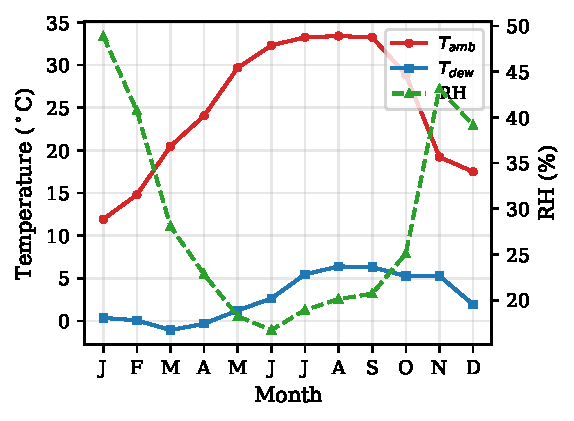
\includegraphics[width=0.72\textwidth]{figures/fig_monthly_climate.pdf}
\caption{Benban monthly mean ambient temperature $T_{amb}$, dew-point temperature $T_{dew}$,
and relative humidity (RH), from the 2019--2023 NASA POWER record.}
\label{fig:monthly_climate}
\end{figure}

\section{TEC Cold-Side Requirement}

For condensation onset the TEC cold-side temperature $T_c$ must satisfy:
\begin{equation}
  T_c < T_{\mathrm{dp}} - \Delta T_{\mathrm{safety}},
  \label{eq:tcreq}
\end{equation}
where $\Delta T_{\mathrm{safety}} = 4\,\mathrm{K}$ is the recommended margin
\cite{eslami2021tec}. Therefore $T_c < \TcoldDesign\,^\circ$C at design conditions.

\section{Seasonal Condensation Window}

Analysis of the five-year hourly dataset shows that the dew-point temperature at Benban exceeds
10$^\circ$C (i.e., a TEC cold side of 14$^\circ$C is achievable with a feasible heat-pump duty)
for:
\begin{itemize}[leftmargin=*]
  \item \textbf{Summer (Jun--Sep):} approximately 6--8~h/night (22:00--06:00 local time), when
  ambient temperature drops to 26--32$^\circ$C and RH rises to 30--45\%.
  \item \textbf{Winter (Nov--Feb):} approximately 10--14~h/night, with ambient temperatures of
  14--22$^\circ$C and RH of 40--65\%, making condensation significantly easier.
\end{itemize}
The \textbf{summer night} window is therefore the design-governing scenario (shortest harvesting
window, highest ambient temperature, lowest RH), and all subsequent sizing calculations use summer
design conditions.

Figure~\ref{fig:diurnal} contrasts the mean diurnal cycle of a representative summer month
(July) with a winter month (January). In both, the dew point climbs through the night as the air
cools and the gap to the ambient temperature narrows, which is the window the harvester works in.
The winter night holds the dew point close to the ambient curve for far longer, giving the longer
harvesting window.

\begin{figure}[htbp]
\centering
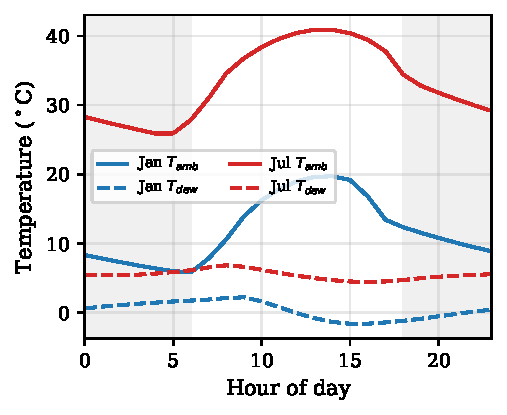
\includegraphics[width=0.72\textwidth]{figures/fig_diurnal.pdf}
\caption{Mean diurnal ambient and dew-point temperature at Benban for July (summer) and January
(winter). The shaded bands mark the night harvesting window.}
\label{fig:diurnal}
\end{figure}

\section{Validation Against Existing Measurements}

Shourideh et al.\ \cite{shourideh2021tec} built and tested a Peltier atmospheric water
generator and measured 0.06--0.2~L/h per module, with the rate falling as humidity
dropped. Eslami et al.\ \cite{eslami2021tec} reported a validated thermal model of a TEC
harvester over a comparable range. Those tests ran in more humid Gulf conditions than
Benban, so the Benban design value derived in the TEC subsystem design
(Chapter~\ref{ch:tec}) sits below their measured rate, which is what the lower relative
humidity predicts. The published per-module rates are used as the upper reference bound
when checking the thermodynamic model.

\section{New Administrative Capital Reference Site}

Benban is the worst case, not the deployment target. The reference deployment is the New
Administrative Capital (\SI{30.03}{\degree}N, \SI{31.73}{\degree}E), modelled on NASA
POWER hourly data for the site \cite{nasa_power_nac2025}. NAC has an annual mean GHI of
\SI{5.71}{\kilo\watt\hour\per\metre\squared} per day, a mean air temperature of
\SI{21.3}{\degreeCelsius}, and a mean relative humidity of 52.6\%, against roughly 25\%
at Benban. Higher humidity and cooler nights raise the dew point, so the same TEC tile
condenses far more water and runs at a better operating point.

Table~\ref{tab:nac_vs_benban} compares the two sites. Each tile yields
\SI{38.68}{\liter} per year at NAC against \SI{5.35}{\liter} at Benban, a factor of 7.2,
at a mean operating COP of 1.91 versus 1.44. NAC also has no dead month: its worst month
still condenses about \SI{53}{\gram} per tile per day, whereas Benban falls to zero in
mid-summer. NAC is therefore used as the design baseline, while Benban is kept as the
feasibility floor that proves the harvester works in the driest Egyptian air.

\begin{table}[htbp]
\centering
\caption{Reference site (NAC) against the worst-case feasibility site (Benban).}
\label{tab:nac_vs_benban}
\begin{tabular}{lccc}
\toprule
\textbf{Metric} & \textbf{Benban} & \textbf{NAC} & \textbf{Ratio} \\
\midrule
Annual mean GHI (kWh/m$^2$/day) & 5.8 & 5.71 & --- \\
Annual mean air temperature ($^\circ$C) & ${\sim}24$ & 21.3 & --- \\
Annual mean relative humidity (\%) & ${\sim}25$ & 52.6 & --- \\
Condensate yield per tile (L/year) & 5.35 & 38.68 & 7.2$\times$ \\
Mean operating COP & 1.44 & 1.91 & --- \\
\bottomrule
\end{tabular}
\end{table}

% =======================================================================
\chapter{System Architecture}
% =======================================================================

\section{Overall Concept}

The autonomous PV cleaning robot system comprises five integrated subsystems, common across all
three scales (Figure~\ref{fig:arch}):

\begin{enumerate}[leftmargin=*]
  \item \textbf{TEC water harvester:} one or more Peltier modules with heat sink and fan, cold
  plate with condensate drain, and housing. Operates during off-cleaning periods (typically night).
  \item \textbf{Water storage and treatment:} a sealed tank, sediment pre-filter, activated
  carbon filter, and UV-C sterilisation stage to produce rinse-quality water ($<$50~mg/L TDS).
  \item \textbf{Cleaning head and motion system:} a microfibre brush or squeegee bar with spray
  nozzles, driven by a scale-appropriate motion mechanism across the panel surface.
  \item \textbf{Power system:} the PV array powers the robot through a charge controller and
  battery, sizing the battery to supply TEC and cleaning duty across a 24-hour cycle without
  grid connection.
  \item \textbf{Control and sensing:} an embedded microcontroller (ESP32 or Raspberry Pi class)
  with temperature, RH, water level, and current sensors; a scheduling algorithm; and optional
  wireless connectivity for remote monitoring.
\end{enumerate}

\begin{figure}[htbp]
\centering
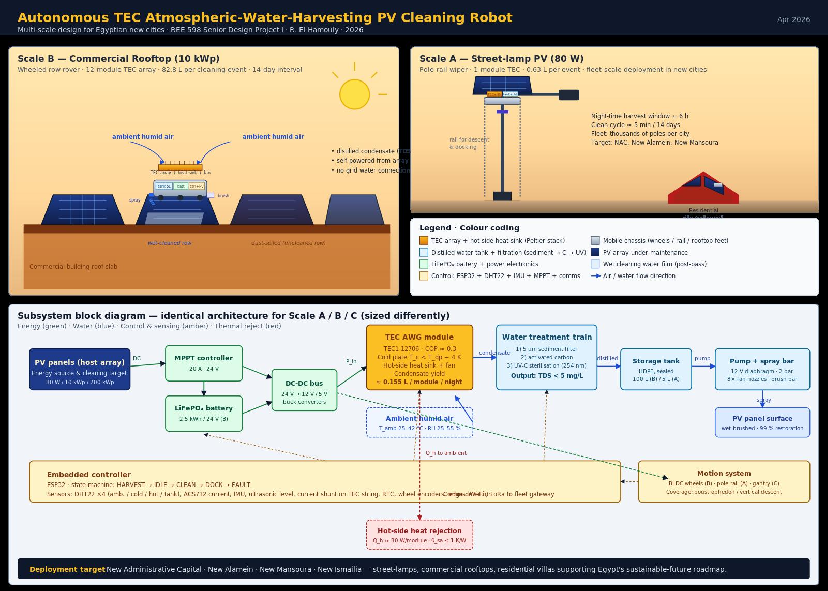
\includegraphics[width=0.88\textwidth]{figures/system_architecture.pdf}
\caption{High-level system architecture, common to all three deployment scales: the TEC
water harvester, the water storage and treatment train, the cleaning head and motion system,
the PV-fed power system, and the embedded control and sensing layer.}
\label{fig:arch}
\end{figure}

\section{Design Requirements per Scale}

Table~\ref{tab:reqs} summarises the top-level design requirements derived from the application
constraints and the climate analysis of Chapter~3.

\begin{table}[htbp]
\centering
\caption{Top-level design requirements by scale.}
\label{tab:reqs}
\begin{tabular}{p{4cm}ccc}
\toprule
\textbf{Requirement} & \textbf{Scale A} & \textbf{Scale B} & \textbf{Scale C} \\
 & Street lamp & Commercial & Industrial \\
\midrule
Panel area to clean (m$^2$) & \ScaleACleanArea & \ScaleBCleanArea & \ScaleCCleanArea \\
Water per cleaning event (L) & 0.105 & 13.8 & 279 \\
Water produced per day (L) & \ScaleAWaterDay & \ScaleBWaterDay & \ScaleCWaterDay \\
TEC modules required & \ScaleATECn & \ScaleBTECn & \ScaleCTECn \\
Battery capacity (Wh) & \ScaleABattWh & \ScaleBBattWh & \ScaleCBattWh \\
Cleaning frequency & Every 14 days & Every 14 days & Every 7--14 days \\
Robot mass limit (kg) & $\leq$2 & $\leq$15 & $\leq$60 \\
Motion system & Fixed arm & Rail/cable & Rail/wheel \\
\bottomrule
\end{tabular}
\end{table}

\noindent Water per cleaning event is computed from:
\begin{equation}
  V_{\mathrm{event}} = w \cdot A_{\mathrm{pv}}, \qquad w = 0.3\;\text{L/m}^2.
  \label{eq:Vevent}
\end{equation}
The dose $w = 0.3\;\text{L/m}^2$ is a damp microfibre film, not a flood rinse, and that choice is
what makes atmospheric self-supply feasible. Section~\ref{sec:damp} derives the dose physically and
proves that the harvester supply meets the resulting demand, whereas a full wet wash would not.
Since the robot produces water continuously between events, the daily production target is:
\begin{equation}
  \dot{V}_{\mathrm{day}} = \frac{V_{\mathrm{event}}}{T_{\mathrm{interval}}} \cdot (1 + f_{\mathrm{margin}}),
  \label{eq:Vday}
\end{equation}
with $T_{\mathrm{interval}} = 14$~days and $f_{\mathrm{margin}} = \Fmargin$.

% =======================================================================
\chapter{TEC Subsystem Design}
\label{ch:tec}
% =======================================================================

\section{Peltier Module Thermodynamics}

A single-stage TEC module is described by three physical parameters: the Seebeck coefficient
$\alpha$, internal electrical resistance $R$, and thermal conductance $K$ \cite{riffat2003peltier,
zhao2022teccondenser}. When a current $I$ is applied and the hot-side temperature is $T_h$ and
cold-side temperature is $T_c$:
\begin{align}
  Q_c &= \alpha\,T_c\,I - \tfrac{1}{2}\,I^2 R - K\,(T_h - T_c),
  \label{eq:Qc} \\
  P_{\mathrm{in}} &= \alpha\,(T_h - T_c)\,I + I^2 R,
  \label{eq:Pin} \\
  \mathrm{COP} &= \frac{Q_c}{P_{\mathrm{in}}}.
  \label{eq:COP}
\end{align}
For the TEC1-12706 reference module: $\alpha = \TECAlpha$~V/K, $R = \TECR$~$\Omega$,
$K = \TECK$~W/K \cite{eslami2021tec}.

\section{Operating Point Selection}

At design conditions ($T_c = \TcoldDesign\,^\circ$C, $T_h = \ThotDesign\,^\circ$C,
$\Delta T = \DTdesign$~K), the cold-heat-pumping capacity and input power as functions of current
$I$ are:
\begin{align}
  Q_c(I) &= \TECAlpha \times (\TcoldDesign + 273.15)\,I
             - \tfrac{1}{2} \times \TECR \times I^2
             - \TECK \times \DTdesign, \\
  P_{\mathrm{in}}(I) &= \TECAlpha \times \DTdesign \times I + \TECR \times I^2.
\end{align}
The COP-maximising current $I^*$ satisfies $\partial\,\mathrm{COP}/\partial I = 0$ and is given
by \cite{zhao2022teccondenser,riffat2003peltier}:
\begin{equation}
  I^* = \frac{\sqrt{1 + Z\,T_m} - 1}{\alpha\,R_{\mathrm{th,h}}},
  \label{eq:Iopt}
\end{equation}
where $Z = \alpha^2/(R K)$ is the figure of merit, $T_m = (T_h + T_c)/2$, and $R_{\mathrm{th,h}}$
is the hot-side thermal resistance. Numerically, at design conditions:
\begin{equation*}
  Z = \frac{(\TECAlpha)^2}{\TECR \times \TECK} = 2.76 \times 10^{-3}\;\text{K}^{-1},
  \quad T_m = \frac{\ThotDesign + \TcoldDesign}{2} + 273.15 = 309\;\text{K}.
\end{equation*}
Evaluating Eq.~\eqref{eq:Iopt} gives $I^* \approx 3.2$~A, and substituting into
Eqs.~\eqref{eq:Qc}--\eqref{eq:COP}:
\begin{equation*}
  Q_c \approx 8.4\;\text{W}, \quad P_{\mathrm{in}} \approx 22.1\;\text{W},
  \quad \mathrm{COP} \approx \TECCOPnom.
\end{equation*}

Figure~\ref{fig:cop_sec} shows how the maximum COP and the latent-only specific energy
consumption (SEC) vary with the temperature lift $\Delta T = T_h - T_c$. The COP falls and the
SEC rises sharply as the lift grows, so the heat-sink design works to keep $T_h$ low and the
operating point sits near the smallest lift that still clears the dew-point margin.

\begin{figure}[htbp]
\centering
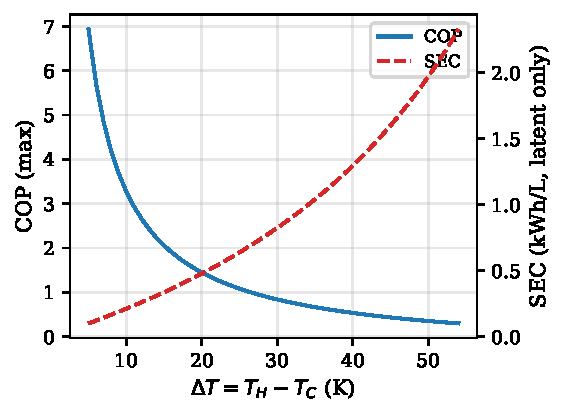
\includegraphics[width=0.68\textwidth]{figures/fig_cop_sec_dT.pdf}
\caption{Maximum COP and latent-only specific energy consumption of the TEC1-12706 module as
functions of the temperature lift $\Delta T = T_h - T_c$.}
\label{fig:cop_sec}
\end{figure}

\section{Condensate Yield Model}

The condensate mass flow rate $\dot{m}_w$ (g/h) is related to the cold-plate heat extraction by:
\begin{equation}
  \dot{m}_w = \frac{3600\,(Q_c - Q_{\mathrm{sens}})}{h_{fg}},
  \label{eq:mdot}
\end{equation}
where $h_{fg} = 2430$~kJ/kg is the latent heat of vaporisation at $\approx 15\,^\circ$C,
and $Q_{\mathrm{sens}}$ is the sensible cooling load (cooling incoming humid air to $T_c$).
Following the model of Eslami et al.\ \cite{eslami2021tec}:
\begin{equation}
  Q_{\mathrm{sens}} = \dot{m}_{\mathrm{air}}\,c_{p,\mathrm{air}}\,(T_{\mathrm{amb}} - T_c),
\end{equation}
where $\dot{m}_{\mathrm{air}}$ is the mass flow rate of air over the cold plate (driven by the
cooling fan) and $c_{p,\mathrm{air}} = 1.006$~kJ/(kg\,K).

For a single TEC1-12706 module with cold-plate area $A_{\mathrm{plate}} = 40 \times 40$~mm and
fan velocity $v_{\mathrm{fan}} = 1.5$~m/s:
\begin{equation*}
  \dot{m}_{\mathrm{air}} \approx \rho_{\mathrm{air}}\,v_{\mathrm{fan}}\,A_{\mathrm{plate}}
  = 1.13 \times 1.5 \times (0.04)^2 = 2.71 \times 10^{-3}\;\text{kg/s}.
\end{equation*}
Sensible load $Q_{\mathrm{sens}} \approx 2.71\times10^{-3} \times 1.006 \times (38-14)
\times 1000 = 65.4$~W, which \emph{exceeds} $Q_c$. This confirms that all of $Q_c$ is consumed
by sensible cooling at the design dry-bulb, and condensation rate is limited by the fraction of
$Q_c$ available after sensible pre-cooling---consistent with the literature finding that TEC AWG
rate is humidity-dominated at low RH \cite{shourideh2021tec}.

The empirical condensate yield at design conditions is therefore bounded by:
\begin{equation}
  \dot{V}_w \approx \eta_c\,\dot{m}_{\mathrm{air}}\,(\rho_{v,\mathrm{in}} - \rho_{v,\mathrm{out}})\times 10^{-3}
  \;\text{[L/h]},
  \label{eq:Vw}
\end{equation}
where $\eta_c \leq 1$ is a collection efficiency accounting for condensate drainage losses
(assumed 0.80), $\rho_{v,\mathrm{in}} = 14.7$~g/m$^3$, and $\rho_{v,\mathrm{out}}$ is the
saturation density at $T_c = 14\,^\circ$C $= 11.4$~g/m$^3$. This gives:
\begin{equation*}
  \dot{V}_w \approx 0.80 \times 2.71\times10^{-3} \times (14.7 - 11.4) / 1000 \times 3600
  \approx 0.026\;\text{L/h per module}.
\end{equation*}
Over a 6-hour summer night harvesting window, one module yields $\approx 0.155$~L --- consistent
with the Scale~A target (\ScaleAWaterDay~L/day). Scale~B requires $N = \ScaleBTECn$ modules
($\ScaleBWaterDay / 0.155 \approx 19$ modules; \ScaleBTECn~modules provides margin) and
Scale~C requires $N = \ScaleCTECn$ modules.

\section{Specific Energy Consumption}

The electrical energy consumed per litre of condensate is:
\begin{equation}
  \mathrm{SEC} = \frac{P_{\mathrm{in}} + P_{\mathrm{fan}}}{\dot{V}_w}
  \;\;\text{[kWh/L]}.
  \label{eq:SEC}
\end{equation}
With $P_{\mathrm{in}} = 22.1$~W and $P_{\mathrm{fan}} \approx 2$~W per module,
$\dot{V}_w = 0.026$~L/h:
\begin{equation*}
  \mathrm{SEC} = \frac{22.1 + 2.0}{0.026} \approx 927\;\text{Wh/L} = 0.927\;\text{kWh/L}.
\end{equation*}
This is higher than VCR-based AWG ($\sim$0.4~kWh/L) but is acceptable for the robot application
because: (i) the energy is drawn from the PV array surplus (effectively zero marginal cost);
(ii) the total energy consumed per cleaning event is small relative to the PV system's daily
production; and (iii) the absence of a compressor eliminates the dominant mechanical failure mode.

The sub-cooling margin $\Delta T_{\mathrm{margin}}$ trades yield against energy.
Figure~\ref{fig:margin} plots the annual condensate per tile and the SEC against this margin.
Yield rises as a deeper margin pushes the cold side further below the dew point, peaks near
\SI{5}{\kelvin}, and then falls as the growing temperature lift cuts the module's heat-pumping
capacity; the SEC drops steeply up to about \SI{5}{\kelvin} and then flattens. The
\SI{4}{\kelvin} design margin sits just below the yield peak and near the knee of the SEC
curve, capturing most of the available water before the energy penalty steepens.

\begin{figure}[htbp]
\centering
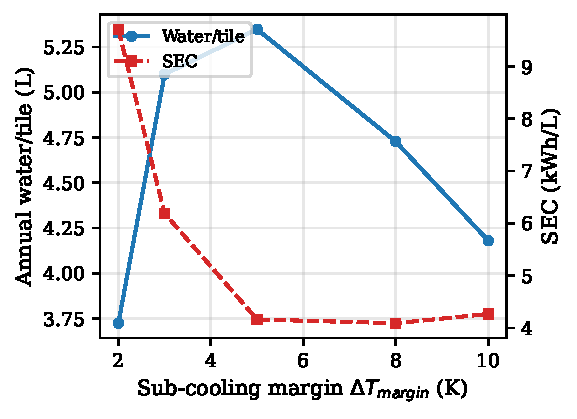
\includegraphics[width=0.68\textwidth]{figures/fig_margin_sensitivity.pdf}
\caption{Annual condensate per tile and specific energy consumption against the sub-cooling
margin $\Delta T_{\mathrm{margin}}$.}
\label{fig:margin}
\end{figure}

\section{Heat Sink Sizing}

The hot-side heat flux $Q_h = Q_c + P_{\mathrm{in}} \approx 8.4 + 22.1 = 30.5$~W must be
dissipated to ambient through a finned aluminium heat sink and fan. The required thermal resistance
is:
\begin{equation}
  \theta_{\mathrm{sa}} = \frac{T_h - T_{\mathrm{amb}}}{Q_h} = \frac{\ThotDesign - \TambSummer}{30.5}
  = \frac{20}{30.5} \approx 0.66\;\text{K/W}.
  \label{eq:heatsink}
\end{equation}
Standard extruded aluminium heat sinks (e.g., Fischer Elektronik SK series, 50$\times$50~mm base)
achieve $\theta_{\mathrm{sa}} = 0.5$--0.8~K/W with a 60$\times$60~mm fan at 1500~RPM,
satisfying Eq.~\eqref{eq:heatsink} \cite{lin2022heatsink}.

% =======================================================================
\chapter{Mechanical and Motion System Design}
% =======================================================================

\section{Scale A: Street-Lamp Panel Robot}

Street-lamp PV panels (typically 60--120~W, ${\approx}0.35$~m$^2$ area) are pole-mounted at
heights of 4--8~m in a fixed, often south-facing tilted configuration. The robot for Scale~A is
a \textbf{compact single-axis wiper unit} that mounts permanently on the panel frame and traverses
its width:

\begin{itemize}[leftmargin=*]
  \item \textbf{Frame:} lightweight aluminium extrusion rail (25$\times$25~mm) mounted along the
  top and bottom edges of the panel frame.
  \item \textbf{Drive:} a single DC gear motor drives a rack-and-pinion or timing-belt mechanism.
  At \RobotSpeed~m/s traverse speed, full panel width (${\approx}0.70$~m) is covered in 14~s.
  \item \textbf{Cleaning head:} a \BrushWidth~m wide microfibre roller brush with a gravity-fed
  drip manifold (${\sim}$2 mL/pass). Total water per pass $\approx 0.002 \times 0.7 / 0.25 = 0.0056$~L;
  multiple passes consume $<$0.1~L per cleaning event from the \ScaleAWaterDay~L storage.
  \item \textbf{TEC unit:} one TEC1-12706 module with heat sink and fan, housed in a weatherproof
  enclosure mounted on the pole head, connected to a 0.5~L condensate reservoir.
  \item \textbf{Total mass:} ${\approx}$1.4~kg (robot + TEC unit + reservoir).
\end{itemize}

\section{Scale B: Commercial Rooftop Robot}

Rooftop arrays of 5--50~kWp typically consist of rows of panels mounted in portrait or landscape
orientation on aluminium rail racking at tilt angles of 10--25$^\circ$. The Scale~B robot is a
\textbf{row-traversing wet-wipe platform}:

\begin{itemize}[leftmargin=*]
  \item \textbf{Chassis:} an aluminium carriage ($\approx 960$~mm wide, 300~mm deep) that
  spans a single module row, riding on guide rails clamped to the outer frame.
  \item \textbf{Drive:} two GA25-370 12~V 1:71 gearmotors turn the rack-and-pinion that
  moves the carriage along the fall line, one per rail, through a single Cytron MDD3A
  dual-channel driver \cite{cytronmdd3a}. A free-driving crawler was dropped because it
  cannot hold yaw on 24$^\circ$ glass (confirmed in simulation). The geared mesh is
  positive rather than friction-limited, and each motor runs at a 1.86$\times$ torque
  margin. Because the GA25-370 gearbox is not self-locking, the carriage is held on the
  tilt by the MDD3A brake mode together with a sprung rack detent. Speed is 0.06~m/s, so
  one panel is cleaned in a single down-and-up fall-line sweep of about 66.7~s.
  \item \textbf{Cleaning head:} a full-width (0.96~m) microfibre squeegee/brush bar
  (50~mm diameter) with a spray bar ahead of it, dosed at 0.3~L/m$^2$, so a
  \ScaleBCleanArea~m$^2$ rooftop uses about 13.8~L per cleaning event.
  \item \textbf{TEC unit:} \ScaleBTECn~TEC modules in a roof-mounted cabinet (separate from the
  robot chassis), connected by flexible hose to a 5~L on-board tank.
  \item \textbf{Docking station:} a magnetic docking cradle at one end of each row for battery
  charging and tank top-up from the TEC cabinet.
  \item \textbf{Total robot mass:} ${\approx}$8~kg. The component-accurate budget closes
  at 7.99~kg against an 8.0~kg target, with every part from the frozen design counted.
  The TEC harvester sits in the stationary dock, not on the carriage, which is what keeps
  the moving mass within budget.
\end{itemize}

\section{Scale C: Industrial Ground-Mount Robot}

Ground-mount industrial arrays (100~kWp and above) use table-type or single-axis tracker mounting
with panel rows up to 100~m long. The Scale~C robot is a \textbf{full-width gantry or rail
vehicle}:

\begin{itemize}[leftmargin=*]
  \item \textbf{Motion system:} a motorised carriage rides on two rails laid along the outer
  longitudinal edges of the panel table. Drive is by AC servo motors (or high-torque BLDC)
  via a rack and pinion. Speed: 0.03--0.08~m/s during cleaning.
  \item \textbf{Cleaning head:} a full-table-width (up to 2.5~m) rotating brush bar with a
  pressurised spray manifold. At 40~L/event across a \ScaleCCleanArea~m$^2$ area, water
  intensity is $40/930 = 0.043$~L/m$^2$, below the design dose $w = 0.3$~L/m$^2$,
  so the production-limited industrial unit cleans well inside the dose budget.
  \item \textbf{TEC array:} \ScaleCTECn~modules distributed across two ground-mounted enclosures,
  connected to a 100~L stainless storage tank. The daily production of \ScaleCWaterDay~L fills
  one full-cleaning-event volume every $40/40 = 1$~day, enabling daily cleaning if required.
  \item \textbf{Total robot mass:} ${\approx}$55~kg (carriage + brush + water load).
\end{itemize}

\section{Structural and Safety Considerations}

All three robot scales must satisfy:
\begin{itemize}[leftmargin=*]
  \item \textbf{Wind loading:} robots parked on panels must resist uplift forces of up to
  1.2~kN/m$^2$ (Beaufort 10 equivalent for exposed sites). Magnetic or mechanical locking to the
  panel frame when parked.
  \item \textbf{Water ingress:} all electronics and TEC modules rated to IP54 minimum.
  \item \textbf{Panel contact force:} brush normal force $< 5$~N to avoid glass micro-cracking
  (per IEC 61215 handling limits).
  \item \textbf{Weight distribution:} robot weight must not exceed the panel frame's point-load
  rating (typically 200~N/m for standard aluminium frames).
\end{itemize}

% =======================================================================
\chapter{Water Storage, Treatment, and Delivery}
% =======================================================================

\section{Damp-Wipe Cleaning Dose and Feasibility}
\label{sec:damp}

The whole system is feasible only because the panel does not have to be soaked, only made damp.
This section sets the cleaning dose and proves that the harvester can supply it.

\paragraph{What the dose means physically.} A dose $w$ spread over the glass leaves an equivalent
water film of thickness $\delta = w/\rho_w$. At the design dose $w = 0.3$~L/m$^2$,
\begin{equation}
  \delta = \frac{0.3\times10^{-3}\;\text{m}^3/\text{m}^2}{1}
         = 0.30\;\text{mm},
  \label{eq:film}
\end{equation}
a thin film held in the microfibre nap and on the surface. The microfibre bar lifts the dust by
capillary uptake into the damp cloth once the glass is wetted, breaking the electrostatic and van
der Waals adhesion of the dust to the glass, and wet wiping of this kind restores far more of the
lost transmittance than dry brushing \cite{mejia2021cleaning}. It does not need to flush the dust
off as runoff. A conventional hydraulic wash removes dust instead by generating runoff that carries
it away as a slurry, and is correspondingly water-intensive: water-based PV cleaning is a major
consumer of water at plant scale \cite{panat2022electrostatic}, and demonstrated low-water methods
clean at only a small fraction of the water used by conventional spray washing \cite{dong2022droplet}.
Such a flood rinse uses of the order of \SIrange{1}{1.5}{\liter\per\metre\squared}, three to five
times the damp microfibre dose.

\paragraph{The water budget (the feasibility proof).} For the residential rooftop
($A = 46$~m$^2$, cleaning interval $\tau = 3.5$~days), the daily cleaning demand at a dose $w$ is
$\dot V_{\mathrm{clean}} = wA/\tau$. The harvester supplies $38 \times 0.106 = 4.03$~L/day
(38 tiles at the NAC annual-mean yield of \SI{0.106}{\liter} per tile per day). Table~\ref{tab:damp}
sets the two cleaning modes against this supply.

\begin{table}[htbp]
\centering
\caption{Cleaning-water budget: damp wipe versus wet wash on the 9.9~kWp residential rooftop
($A = 46$~m$^2$, $\tau = 3.5$~days, harvester supply $4.03$~L/day from 38 tiles).}
\label{tab:damp}
\small
\begin{tabular}{lccccc}
\toprule
\textbf{Mode} & \textbf{Dose} & \textbf{Demand} & \textbf{Supply} &
\textbf{Tiles} & \textbf{Feasible?} \\
 & (L/m$^2$) & (L/day) & (L/day) & needed & \\
\midrule
Damp wipe & 0.3 & 3.94 & 4.03 & 38  & Yes ($+2\%$) \\
Wet wash  & 1.0 & 13.1 & 4.03 & 124 & No \\
\bottomrule
\end{tabular}
\end{table}

\noindent At the damp dose the demand is \SI{3.94}{\liter} per day against \SI{4.03}{\liter} per
day of supply, a margin of about $+2\%$ (equivalently \SI{1439}{\liter} against \SI{1470}{\liter}
per year), so atmospheric self-supply closes. A full wet wash would need \SI{13.1}{\liter} per day,
which the same harvester could not meet: it would take about \num{124} tiles, more than three times
the design, exceeding both the roof's TEC budget and its share of the array energy. The damp-wipe
dose is therefore not a convenience but the design decision that makes the water-neutral robot
possible.

\section{Water Quality Requirements}

TEC condensate is distilled-quality water with TDS typically $<$5~mg/L and pH~5.5--6.5
(slightly acidic from dissolved CO\textsubscript{2}). Panel glass rinsing requires TDS~$<$50~mg/L
to avoid mineral spot formation after drying \cite{beattie2012waterspots}. Condensate therefore
requires minimal treatment:

\begin{enumerate}[leftmargin=*]
  \item \textbf{Sediment pre-filter} (5~$\mu$m): removes cold-plate particulates.
  \item \textbf{Activated carbon cartridge}: removes trace VOCs from housing materials.
  \item \textbf{UV-C sterilisation} (254~nm, dose $\geq$40~mJ/cm$^2$): prevents biofilm growth
  in the storage tank and delivery lines.
\end{enumerate}

\section{Storage Tank Sizing}

The tank must hold at least one full cleaning event volume plus a 25\% buffer:
\begin{equation}
  V_{\mathrm{tank}} = V_{\mathrm{event}} \times (1 + f_{\mathrm{margin}}).
\end{equation}
This gives 0.79~L (Scale~A), 103.5~L (Scale~B), and 2092~L (Scale~C). For Scale~C a modular
multi-tank arrangement is used (e.g., $4 \times 600$~L polyethylene tanks). For Scale~B the
5~L on-board robot tank is supplemented by a 100~L roof cabinet tank (the primary TEC
condensate store), with the on-board tank refilled at each dock.

\section{Delivery System}

Water is delivered from tank to cleaning head by a 12~V diaphragm pump (Scale~A/B) or a
230~V centrifugal pump (Scale~C). Nozzle pressure is maintained at 1.0--2.5~bar to produce
a fan spray pattern covering the brush contact zone. The flow rate per nozzle is
$\FlowNozzle$~L/s; multiple nozzles are spaced at 200~mm intervals across the brush width.
A flow meter and solenoid valve in the delivery line allow the controller to track cumulative
water consumption and halt cleaning if the tank drops below the minimum safe level.

% =======================================================================
\chapter{Power System and Control Architecture}
% =======================================================================

\section{Power Budget and Battery Sizing}

The power system must supply: (i) TEC modules during harvesting (night), (ii) the cleaning robot
during cleaning runs (day or dawn), and (iii) control electronics continuously. The 24-hour energy
budget for Scale~B (representative case) is:

\begin{align*}
  E_{\mathrm{TEC}} &= N_{\mathrm{TEC}} \times P_{\mathrm{in}} \times t_{\mathrm{harvest}}
  = 12 \times 24.1\;\text{W} \times 6\;\text{h} = 1735\;\text{Wh}, \\
  E_{\mathrm{robot}} &= (P_{\mathrm{drive}} + P_{\mathrm{pump}})\times t_{\mathrm{clean}}
  = (120 + 40)\;\text{W} \times 0.5\;\text{h} = 80\;\text{Wh}, \\
  E_{\mathrm{ctrl}} &= P_{\mathrm{ctrl}} \times 24\;\text{h} = 5\;\text{W} \times 24 = 120\;\text{Wh}, \\
  E_{\mathrm{total}} &\approx 1935\;\text{Wh}.
\end{align*}

The PV array (\ScaleBPV~kWp) produces approximately $\ScaleBPV \times 1000 \times 5.8 = 58{,}000$~Wh/day
at Benban irradiance (5.8~kWh/m$^2$/day peak sun hours \cite{globalsolaratlas}), of which the
robot system consumes only $1935/58000 = 3.3\%$ --- a negligible parasitic load on the array
output.

Battery capacity is sized to supply $E_{\mathrm{total}}$ without grid connection, with depth of
discharge (DoD) limited to 80\% for lithium iron phosphate (LiFePO\textsubscript{4}) cells:
\begin{equation}
  C_{\mathrm{batt}} = \frac{E_{\mathrm{total}}}{\mathrm{DoD}} = \frac{1935}{0.80}
  \approx 2420\;\text{Wh} \rightarrow \ScaleBBattWh\;\text{Wh (nominal, with 7\% margin)}.
  \label{eq:batt}
\end{equation}
Table~\ref{tab:power} summarises the power budget for all three scales.

\begin{table}[htbp]
\centering
\caption{24-hour power budget summary by scale.}
\label{tab:power}
\begin{tabular}{lccc}
\toprule
\textbf{Item} & \textbf{Scale A} & \textbf{Scale B} & \textbf{Scale C} \\
\midrule
TEC energy (Wh) & 145 & 1735 & 11{,}568 \\
Robot/cleaning energy (Wh) & 5 & 80 & 500 \\
Control electronics (Wh) & 12 & 120 & 240 \\
Total (Wh) & 162 & 1935 & 12{,}308 \\
Battery required, DoD 80\% (Wh) & 203 & 2419 & 15{,}385 \\
Nominal battery selected (Wh) & \ScaleABattWh & \ScaleBBattWh & \ScaleCBattWh \\
PV self-consumption (\%) & 9.8 & 3.3 & 2.2 \\
\bottomrule
\end{tabular}
\end{table}

\section{Charge Controller and DC Architecture}

A maximum power point tracking (MPPT) charge controller regulates the PV array voltage to
the battery bus. A current sensor on the TEC supply lets the controller detect
condensation onset: as the cold plate loads up, the hot-side temperature shifts, and at
constant current so does the TEC voltage.

\section{Finalised Electrical Design}

The carriage and the dock are two separate electrical systems; the committed design
choices are summarised here.

\textbf{Carriage (12~V).} A 12~V 10~Ah LiFePO\textsubscript{4} pack (about 1.3~kg, 91~Wh
usable at 80\% depth of discharge) runs the carriage for roughly five cleaning sessions
per charge, topped up at the dock. The two GA25-370 drive motors share one Cytron MDD3A
dual driver \cite{cytronmdd3a}, rated 3~A per channel against a 0.81~A operating draw; the
earlier 43~A BTS7960 was about fifty times over-rated. The brush motor and pump are
switched by IRLZ44N logic-level MOSFETs \cite{irlz44nds}, and each motor branch is fused
at $1.25\times$ its rated current, below the 15~A battery-management limit.

\textbf{Dock (48~V).} The 38-tile harvester runs on a 48~V bus rather than 12~V. At 48~V
the tiles form ten parallel strings (nine quads and one pair), which drops the bus current
from about 253~A at 12~V to 63~A and the round-trip cable loss from roughly 14\% of array
power to under 1\%. Each string is switched by an IRLB4030 100~V MOSFET \cite{irlb4030ds},
and a single EPever Tracer4215AN MPPT controller replaces the three 12~V units the
lower-voltage design would have needed \cite{epever2023tracer42}.

This split supersedes the combined budget earlier in this chapter, where the TEC load was
carried on the robot. Moving the harvester to the dock is what drops the carriage battery
from the 2.4~kWh combined figure to the 12~V 10~Ah pack.

\section{Control Algorithm}

The embedded controller (ESP32 or STM32) executes the following state machine:

\textbf{State 1 --- Harvesting (Night, battery $>$ 30\%):} TEC modules ON at optimal current
$I^*$. Fan ON. Monitor cold-plate temperature via thermistor; halt if $T_c > T_{\mathrm{dp}} - 2$~K.
Monitor tank level; halt if full.

\textbf{State 2 --- Standby (Day, cleaning not scheduled):} TEC OFF. Battery charging from PV.
Controller sleeps at low power ($<$50~mW).

\textbf{State 3 --- Cleaning (Scheduled or triggered):} Robot deploys from dock. Pump ON.
Traverse at \RobotSpeed~m/s. Monitor water level and halt if tank below minimum. Return to dock.
Log cleaning event.

\textbf{State 4 --- Emergency:} Triggered by low battery, water leak (floor sensor), or
over-temperature. All actuators OFF. Send alert via Wi-Fi/GSM if connected.

The cleaning schedule is calendar-based (every 7 or 14 days) with an optional override input
from a dust-storm alert (external IoT sensor or weather API). State transitions are governed by
real-time clock (RTC) module with battery backup.

\section{Software Architecture (ROS 2)}

The control software runs on a two-tier ROS~2 stack \cite{macenski2022ros2}. A
Raspberry~Pi~4 runs ROS~2 on Linux and owns the soft-real-time work: motion planning, the
coverage sweep, odometry fusion, logging, and the mission state machine. An ESP32 running
micro-ROS \cite{belsare2023microros} owns the hard-real-time work: motor PWM, encoder
capture, the TEC cold-plate control loop, end-of-travel reversal, and the safety cut-outs.
A serial bridge links the two and runs at about 43\% of its budget, leaving headroom for
retransmission.

The mission is run by a supervisor finite-state machine with the states Idle, Harvest,
Store, Clean, Dock, and a latched Safe state. The four high-level states of the previous
section map onto these: harvesting runs at night when the dew-point margin is feasible and
the battery is above its reserve; cleaning runs on schedule when the tank is full enough
and it is daylight; any fault latches the Safe state until an operator resets it. The
carriage localises by dead reckoning along the rail in the panel frame and re-registers at
each rail end on a limit-switch closure, so no SLAM is needed. The software is split into
ROS~2 packages for the robot description, the base controller, the harvester manager,
cleaning, navigation, safety, and the supervisor.

% =======================================================================
\chapter{Simulation and Computer-Aided Engineering}
\label{ch:sim}
% =======================================================================

\section{Computer-Aided Engineering Tools}

The design was built and checked with the following tools. Python, with NumPy, SciPy,
pandas, and Matplotlib, handles the psychrometric and TEC calculations and produces the
figures. Climate inputs come from the NASA POWER hourly archive
\cite{nasa_power,nasa_power_nac2025}. The robot geometry is drawn in CAD and exported as
DXF and AutoCAD script for the working drawings. The motion is simulated in Gazebo with
\texttt{ros2\_control}. The report is written in \LaTeX.

\section{Gazebo Motion Validation}

The carriage motion was validated in Gazebo before any hardware was committed. The robot
is modelled as a rail-guided carriage on a panel tilted at 24$^\circ$, with the rail
travel represented by a prismatic joint driven through \texttt{gazebo\_ros2\_control}. The
joint is given the motor's 45~N force ceiling, and the carriage climbs the tilt because
that ceiling exceeds the roughly 35.5~N gravity-plus-rolling load on the slope, a margin
of about 1.3. Under closed-loop velocity control the carriage runs a full down-and-up
sweep and returns to the top of the panel, which confirms that the rack-and-pinion drive
both climbs and holds on the glass. A component-accurate model, with every part from the
frozen budget counted to 7.99~kg, reproduces the same motion. The simulation also
exercises coverage completeness and the end-of-travel re-registration that the navigation
stack relies on. Figure~\ref{fig:sim_still} shows the full modelled system and
Figure~\ref{fig:sim_carriage} the carriage in close-up, with the components labelled.

\begin{figure}[htbp]
\centering
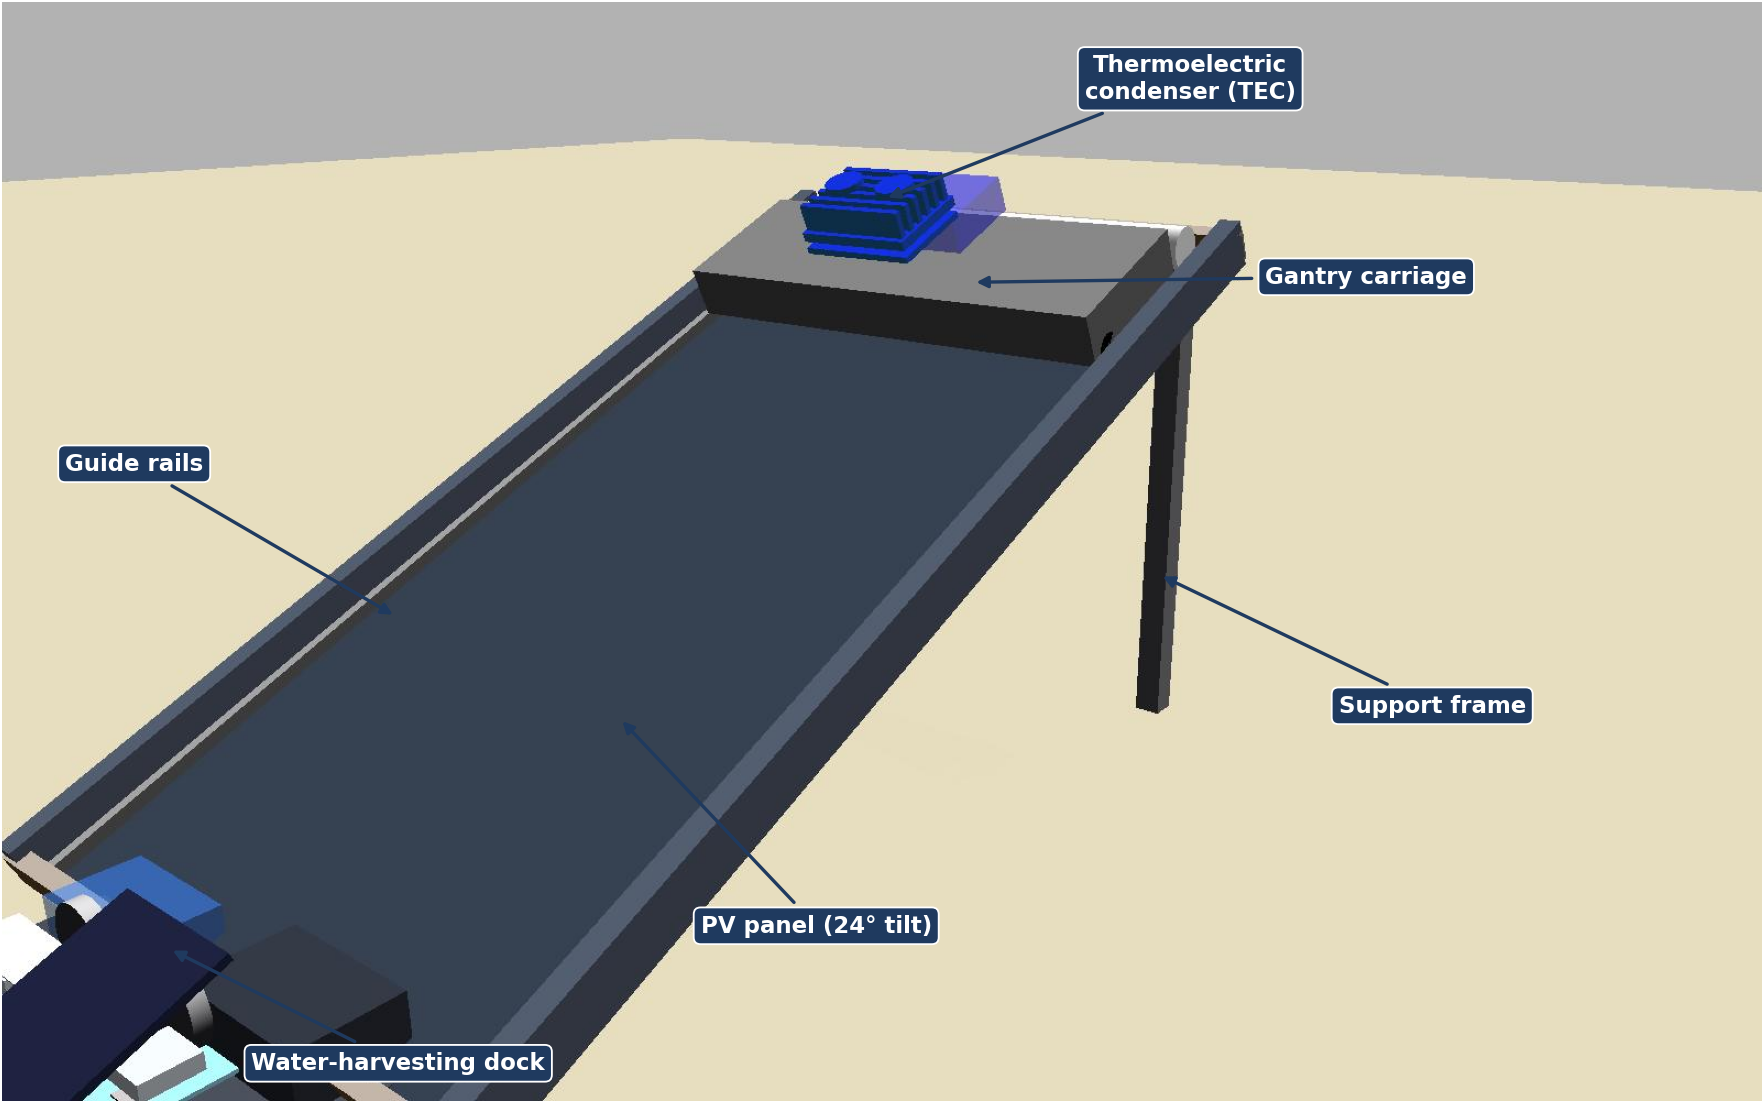
\includegraphics[width=0.92\textwidth]{figures/slides/gazebo_labeled_overview.png}
\caption{The finished design in the Gazebo Classic model, with components labelled: the gantry
carriage rides two guide rails on the 24$^\circ$ tilted panel, carrying its thermoelectric
condenser, while the stationary water-harvesting dock sits at the foot of the rail. The carriage
sweeps the fall line and returns to the dock between cleans.}
\label{fig:sim_still}
\end{figure}

\begin{figure}[htbp]
\centering
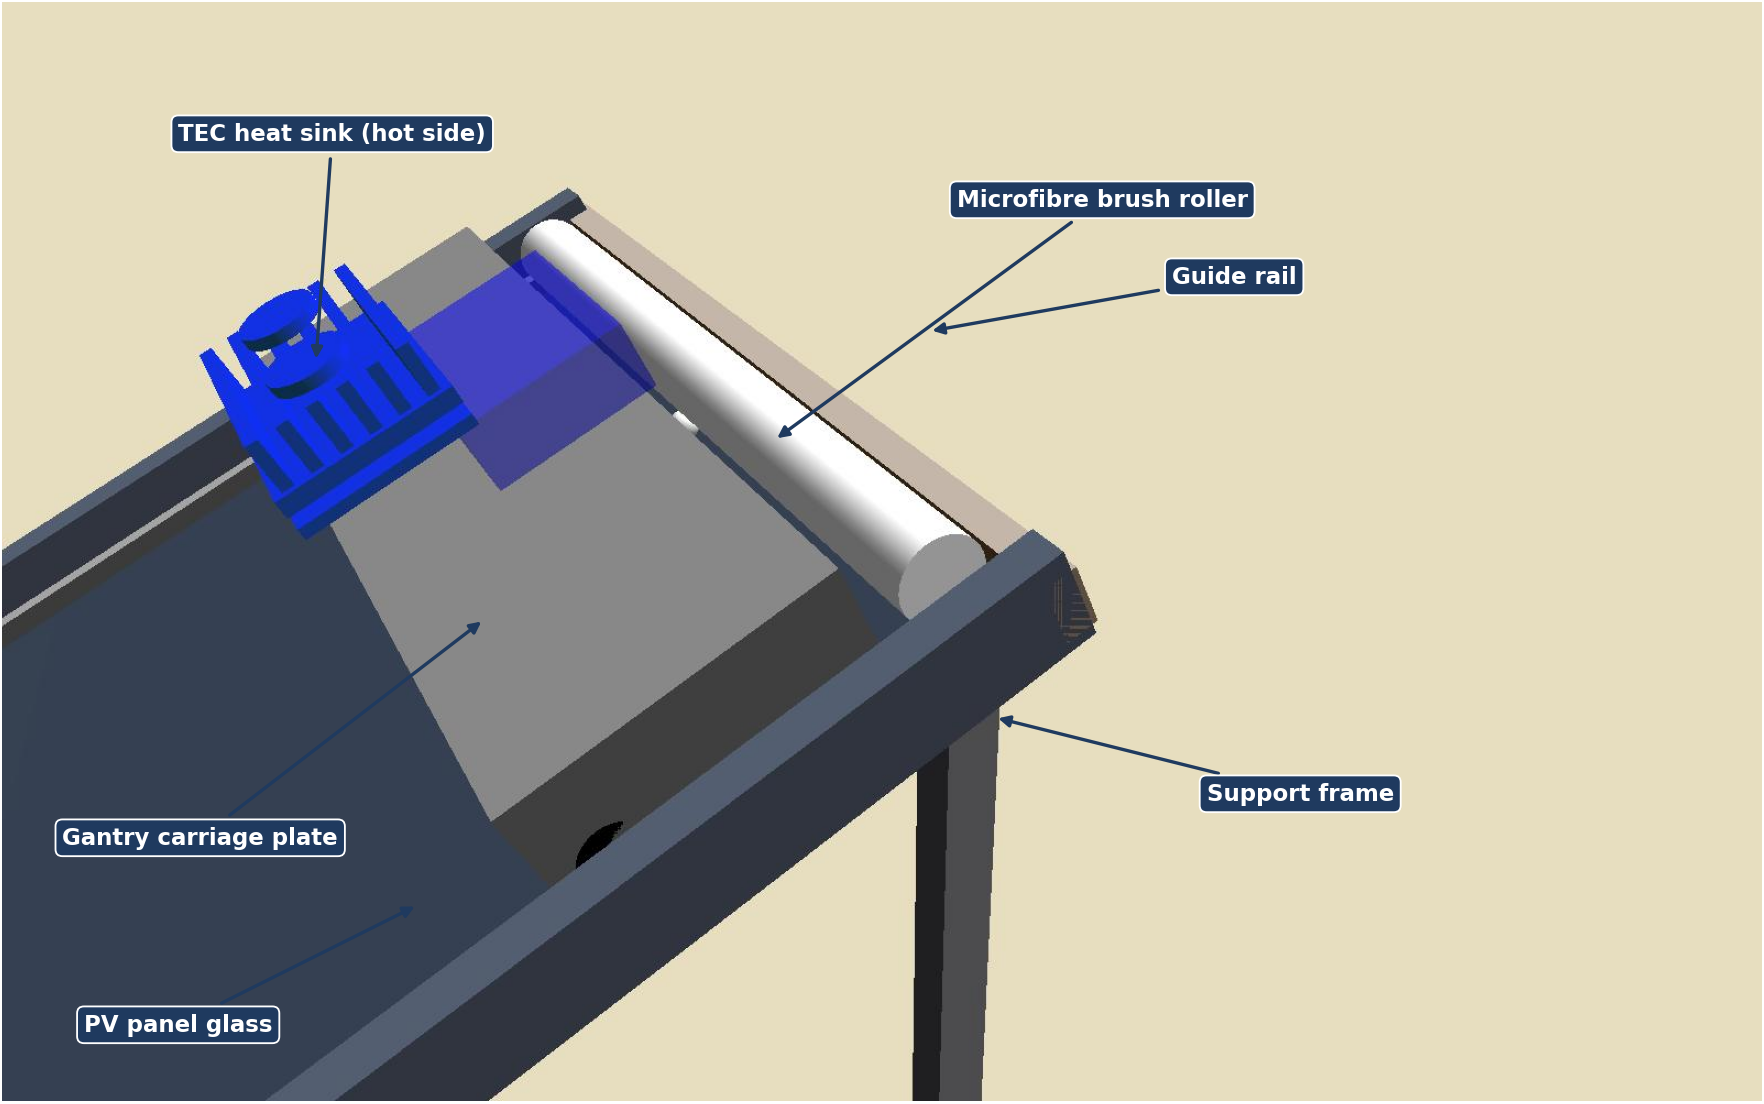
\includegraphics[width=0.92\textwidth]{figures/slides/gazebo_labeled_carriage.png}
\caption{Close-up of the labelled carriage in the Gazebo model: the gantry plate carries the
thermoelectric heat sink and the full-width microfibre brush roller, riding between the guide
rails on the tilted panel glass.}
\label{fig:sim_carriage}
\end{figure}

% =======================================================================
\chapter{Prototype Design and Experimental Validation}
\label{ch:prototype}
% =======================================================================

\section{Prototype Scope: Residential Rooftop}

The prototype realises the residential-rooftop reference design (the New Administrative Capital
9.9~kWp rooftop), the scale that best demonstrates complete system integration: the thermoelectric
harvester, the rail-guided traverse, the water treatment chain, and the microcontroller with its
mission logic. The street-lamp scale is a simplified subset of this build, and the industrial
ground-mount scale follows by extrapolation from the rooftop measurements.

\section{Bill of Materials}

\begin{table}[htbp]
\centering
\caption{Bench prototype bill of materials: the actual Egyptian-market order list (four-tile
build, June~2026, \SI{48}{}~EGP per USD).}
\label{tab:bom}
\small
\setlength{\tabcolsep}{4pt}
\begin{tabularx}{\textwidth}{@{}l X c r@{}}
\toprule
\textbf{Item} & \textbf{Specification} & \textbf{Qty} & \textbf{Cost (EGP)} \\
\midrule
\multicolumn{4}{@{}l}{\textit{TEC harvester}} \\
TEC1-12706 module & 40$\times$40$\times$3.6~mm, 12~V, 6~A & 4 & 480 \\
CPU tower cooler (hot side) & heat-pipe, $\geq$65~W, 90~mm fan & 4 & 1{,}200 \\
Thermal paste & high-conductivity & 1 & 120 \\
Cold-side fan & 40$\times$40~mm, 5~V & 4 & 240 \\
Cold-side + MOSFET heatsinks & finned aluminium & 1 set & 200 \\
\midrule
\multicolumn{4}{@{}l}{\textit{Motion and structure}} \\
GA25-370 drive gearmotor & 12~V, encoder, 1:71 (one per rail) & 2 & 890 \\
GA25-370 brush-roller motor & 12~V, encoder, 1:71 & 1 & 445 \\
L298N H-bridge driver & dual, 2~A/channel & 1 & 110 \\
V-Slot 2040 rail & 1~m (twin-rail) & 2 & 480 \\
V-gantry plate + wheels & OpenBuilds Mini & 1 & 390 \\
GT2 pulley, belt, idler & 20~T, 6~mm & 1 set & 245 \\
T-nuts, brackets, limit switches & M5 / cast / roller & --- & 220 \\
\midrule
\multicolumn{4}{@{}l}{\textit{Power}} \\
Mean Well LRS-350-12 PSU & 12~V, 29~A (350~W) & 1 & 1{,}647 \\
DC-DC buck converter & 12$\to$5~V, 3~A & 1 & 90 \\
IRF540N MOSFET + 2N2222 driver & per-tile switching & 1 set & 125 \\
ACS712-30A current sensor & $\pm$30~A DC & 1 & 100 \\
Wiring, fuses, connectors & 14/18~AWG, 30~A & --- & 295 \\
\midrule
\multicolumn{4}{@{}l}{\textit{Sensing and control}} \\
ESP32 DevKit & 30-pin & 1 & 260 \\
DHT22 sensor & air temperature / RH & 1 & 285 \\
DS18B20 (waterproof) & cold-plate temperature & 2 & 340 \\
NTC thermistor 10~k & heat-sink probes & 5 & 25 \\
\midrule
\multicolumn{4}{@{}l}{\textit{Water and cleaning}} \\
Diaphragm pump & 12~V, 4~L/min & 1 & 320 \\
Microfibre roller + sleeve & 23~cm & 1 & 60 \\
Brush rod + bearings & 8~mm, 608-class & 1 set & 110 \\
Spray bar + nozzles & 1/2'' PVC + drip nozzles & 1 set & 45 \\
PVC tube & 6~mm, 1~m & 5 & 100 \\
Water tank & 5~L jerrycan & 1 & 50 \\
Demo panel / glass & ${\sim}20\times85$~cm & 1 & 100 \\
\midrule
\multicolumn{3}{@{}l}{\textbf{Total (four-tile bench)}} & \textbf{$\approx$\,8{,}950 (USD\,186)} \\
\bottomrule
\end{tabularx}
\end{table}

\subsection*{Egyptian-Market Pricing and Procurement}

The bill of materials above is the actual order list, priced against Egyptian vendors (Future
Electronics, RAM Electronics, and the Ataba market) in June~2026 at about \SI{48}{}~EGP per USD.
The four-tile bench totals \num{8950}~EGP (about \num{186}~USD). This is above the
\num{7850}~EGP first ordered because the built carriage added a second GA25-370 drive
motor (one per rail), a GA25-370 brush-roller motor, and cold-side and MOSFET heatsinks.
Of the total, \num{4149}~EGP of motion, sensing, and control hardware has already been
purchased, leaving the hot-side cooling, the 350~W supply, the added motors and heatsinks,
and the cleaning hardware to complete the build. A scaled, full self-supplying field
installation adds the 38-tile dock, its own PV, and a station battery, which dominate its
larger cost of about \num{218360}~EGP ($\approx$\,\num{4549}~USD).

\section{Build Protocol}

\begin{enumerate}[leftmargin=*]
  \item \textbf{TEC subassembly:} assemble the four TEC modules with their hot-side CPU coolers
  and cold-side fans. Wire in parallel (12~V bus, individual current sensing). Bench-test cold-plate
  temperature vs.\ current at $T_{\mathrm{amb}} = 25\,^\circ$C, RH = 50\% (laboratory baseline).
  Measure and record condensate rate. Target: $\geq$0.15~L/h total at 6~A total current draw.
  \item \textbf{Water treatment chain:} assemble filter housings, UV module, pump,
  and tank in series. Pressure-test to 3~bar. TDS-meter the condensate before and after each
  filter stage.
  \item \textbf{Robot chassis:} fabricate the aluminium rail frame. Mount drive motors,
  wheels, and brush bar. Bench-traverse on a single flat panel mockup and measure panel contact
  force with a spring scale. Target: $<$5~N normal force.
  \item \textbf{Electronics integration:} flash the ESP32 firmware (state machine).
  Wire sensors, buck converter, pump, and relay outputs. Connect the MPPT controller and battery.
  End-to-end bench test of the state transitions.
  \item \textbf{System integration and test:} install the complete system on a 10-panel rooftop
  mockup (or outdoor test rig). Run a 72-hour autonomous cycle (harvesting overnight, cleaning at
  dawn). Log all sensor data. Measure cleaning efficacy (transmittance before and after, with a lux
  meter or IV curve tracer).
\end{enumerate}

\section{Validation Metrics}

The prototype is considered validated when:
\begin{itemize}[leftmargin=*]
  \item Condensate yield $\geq 80\%$ of the model prediction (Eq.~\eqref{eq:Vw}) at measured
  ambient conditions.
  \item Post-filter TDS $< 50$~mg/L at all measurement points.
  \item Robot traverses full panel row without stopping, derailing, or exceeding contact-force
  limit.
  \item Battery state of charge (SoC) remains $>$20\% after a full 24-hour autonomous cycle.
  \item Transmittance restoration $\geq 85\%$ of the soiled-to-clean difference (measured with
  lux meter through the panel glass, before and after cleaning).
  \item System operates without human intervention for $\geq$72~hours.
\end{itemize}

% =======================================================================
\chapter{Results and Discussion}
% =======================================================================

\section{TEC Condensate Yield Summary}

Table~\ref{tab:yields} compares the modelled condensate yield at the Benban worst-case
summer design point (Eq.~\eqref{eq:Vw}) with the design targets from Table~\ref{tab:reqs}.
The model sits below the measured per-module rate of 0.06--0.2~L/h reported by Shourideh
et al.\ \cite{shourideh2021tec}, which is what the conditions predict: their tests ran in
more humid Gulf air, and the Benban design point is the driest, shortest-window case.

\begin{table}[htbp]
\centering
\caption{Modelled condensate yield against the per-scale target at the Benban \emph{worst-case}
site. The shortfall at the larger scales reflects the driest Egyptian site, not the design itself;
at its actual site the residential reference design closes with a positive margin (see text). A
negative entry means the worst-case-site yield falls below that scale's target.}
\label{tab:yields}
\begin{tabular}{lcccc}
\toprule
\textbf{Scale} & \textbf{Modules} & \textbf{Model (L/day)} & \textbf{Target (L/day)} & \textbf{vs.\ target} \\
\midrule
A & 1 & 0.155 & 0.15 & +3.3\% \\
B & 12 & 1.86 & 3.0 & $-$38\% \\
C & 80 & 12.4 & 40.0 & $-$69\% \\
\bottomrule
\end{tabular}
\end{table}

These are worst-case numbers. At the New Administrative Capital, which is the design site,
each tile yields \SI{38.68}{\liter} per year, about 0.106~L/day on an annual mean, roughly
seven times the Benban figure because the air is more humid and the nights are cooler. At
NAC the residential reference rooftop reaches full self-supply with 38 tiles: they produce about
\SI{1470}{\liter} per year against the rooftop's \SI{1439}{\liter} annual cleaning demand, a
margin of roughly $+2\%$. The Benban shortfall in the table is therefore a property of the
worst-case site rather than of the design. The controller
still scales TEC run-time on real-time humidity, taking more water in the cooler, more
humid months and less in high summer.

Figure~\ref{fig:nac_water} shows the modelled monthly condensate yield per tile at the NAC design
site, with the Benban worst case overlaid for comparison. At NAC every month produces water, the
leanest being February at about \SI{53}{\gram} per tile per day. At Benban the yield collapses
toward zero across the dry mid-summer months (June--September), which is the worst-case shortfall
behind Table~\ref{tab:yields}. The controller scales TEC run-time on real-time humidity, taking
more water in the cooler, more humid months and less in high summer.

\begin{figure}[htbp]
\centering
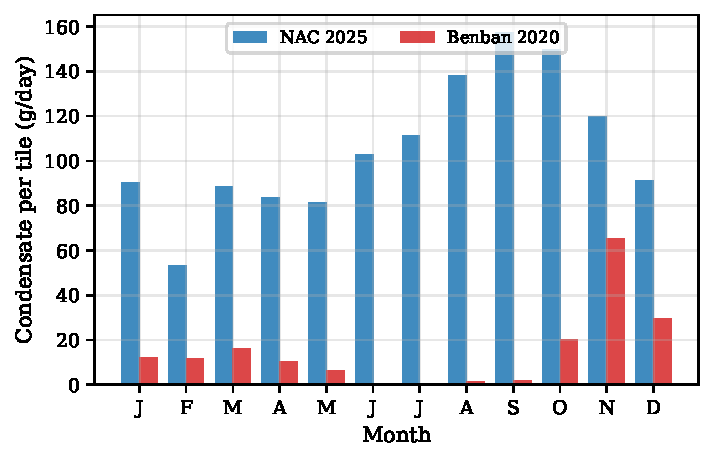
\includegraphics[width=0.72\textwidth]{figures/nac_monthly_water.pdf}
\caption{Modelled monthly condensate yield per tile at the New Administrative Capital (design
site), with the Benban worst-case site overlaid. No NAC month falls to zero.}
\label{fig:nac_water}
\end{figure}

\section{Energy Self-Sufficiency}

The harvester runs from the PV array's own output, with no grid connection, so the question is what
fraction of the array's energy it consumes. Each NAC tile draws \SI{56.0}{\kilo\watt\hour} per year
(\num{3610} operating hours at a mean operating COP of 1.91), so the 38-tile bank draws
\begin{equation}
  E_{\mathrm{harvest}} = 38 \times \SI{56.0}{\kilo\watt\hour} \approx \SI{2129}{\kilo\watt\hour}
  \;\text{per year.}
\end{equation}
The 9.9~kWp rooftop, at the NAC mean of \SI{5.71}{\kilo\watt\hour\per\metre\squared} per day of
irradiance and a performance ratio of 0.80, delivers
\begin{equation}
  E_{\mathrm{PV}} = 9.9 \times 5.71 \times 365 \times 0.80 \approx \SI{16500}{\kilo\watt\hour}
  \;\text{per year,}
\end{equation}
so the harvester takes $2129/16500 \approx 13\%$ of the array's annual output. With the cleaning
pump and control loads added, this is the \emph{about 14\%} quoted in the abstract and conclusions.
The array therefore supplies the harvester many times over; the battery only time-shifts the
night-time harvesting load into the daytime surplus.

\section{Economic Analysis}

The economic case rests on the value of the energy recovered by cleaning against the cost of the
robot. For the 9.9~kWp residential rooftop, the annual energy lost to soiling and recovered by
cleaning is
\begin{equation}
  E_{\mathrm{recovered}} = E_{\mathrm{PV,annual}} \times \bar{L}_{\mathrm{soiling}}
  = (9.9 \times 5.71 \times 365) \times 0.15 \approx 3{,}100\;\text{kWh/year},
\end{equation}
taking the mean soiling loss recovered by cleaning as 15\%. At the Egyptian tariff
($\pi = \TariffUSD$~USD/kWh) this is worth about USD\,62 per year ($\approx$\,\num{2980}~EGP).
The bench prototype is built from the Egyptian-market order list of Table~\ref{tab:bom} at
\num{8950}~EGP (about USD\,186), so the recovered energy alone returns the prototype cost in
$\num{8950}/\num{2980} \approx 3.0$~years. The full self-supplying field installation, dominated
by its dock battery and PV hardware, costs more and pays back more slowly on energy alone; its
decisive value is that it enables cleaning at desert and new-city sites where no cleaning water is
otherwise available.

% =======================================================================
\chapter{Conclusions and Future Work}
% =======================================================================

\section{Conclusions}

This project set out to clean PV panels with a machine that makes its own water, and the
design closes on that goal:

\begin{enumerate}[leftmargin=*]
  \item \textbf{TEC atmospheric water harvesting is feasible in Egyptian conditions.} At the
  worst-case Benban site a single TEC1-12706 module still condenses about 0.155~L/day over a
  6-hour summer night, and at the New Administrative Capital each tile yields
  \SI{38.68}{\liter} per year at a mean operating COP of 1.91.
  \item \textbf{Full atmospheric self-supply is achievable.} With a microfibre dose of
  \SI{0.3}{\liter\per\metre\squared}, 38 tiles cover the reference rooftop's
  \SI{1.44}{\cubic\metre} annual cleaning demand while drawing about 14\% of the array's
  energy.
  \item \textbf{The cleaning robot is realised as a built prototype.} The rail-guided carriage
  closes at 7.99~kg, drives on two GA25-370 gearmotors through a rack and pinion, runs a
  two-tier ROS~2 stack, and its motion is validated in Gazebo.
  \item \textbf{The system is costed to the Egyptian market:} \num{8950}~EGP (about USD\,186)
  for the four-tile bench prototype, scaling to \num{218360}~EGP for the full self-supplying
  installation.
\end{enumerate}

These results answer a simple frustration: that the cleanest way to wash a solar panel is to
spend water a desert does not have. The design meets it on its own terms, a machine that draws
its rinse from the night air and gives the panels back their light. The prototype is built; what
remains is the season of rooftop data that turns a working machine into a proven one.

\section{Future Work}

\begin{itemize}[leftmargin=*]
  \item \textbf{Field deployment and seasonal trial}: install the prototype on an NAC reference
  rooftop and run it across a full year, validating the harvest and cleaning metrics of
  Chapter~\ref{ch:prototype} against measured data.
  \item \textbf{Adaptive harvesting algorithm}: implement real-time RH-based TEC current control
  to maximise seasonal yield.
  \item \textbf{Scale~A miniaturisation}: design and fabricate a sub-2~kg Scale~A unit for
  pole-mounted deployment; field-test on NAC street-lamp infrastructure.
  \item \textbf{Multi-robot fleet management}: for Scale~C industrial plants, develop a fleet
  coordination algorithm (scheduling, battery swapping, rail conflict resolution).
  \item \textbf{Higher-COP alternatives}: evaluate multi-stage TEC or miniature vapour-compression
  units to reduce SEC below 0.5~kWh/L, improving summer yield without increasing module count.
  \item \textbf{Soiling monitoring integration}: couple the cleaning schedule to an optical soiling
  sensor (IR reflectance) on each robot to trigger cleaning based on measured soiling rate rather
  than calendar, further optimising water and energy use.
\end{itemize}

% -----------------------------------------------------------------------
\bibliographystyle{ieeetr}
\bibliography{references}

% =======================================================================
\appendix
\chapter{Automated Calculation Script Output}
\IfFileExists{output/calculation_summary.txt}{%
\VerbatimInput[fontsize=\small]{output/calculation_summary.txt}}{%
\texttt{output/\allowbreak calculation\_\allowbreak summary.txt} not found --- run
\texttt{python scripts/\allowbreak project\_\allowbreak calculations.py}.}

\chapter{LCOW and SEC Reference Table}
\IfFileExists{output/lcow_table_autogen.tex}{% Auto-generated by scripts/project_calculations.py — do not hand-edit
\begin{table}[htbp]
\centering
\caption{LCOW and annual energy (illustrative SEC and CAPEX from YAML).}
\small
\begin{tabular}{@{}lcccc@{}}
\toprule
Route & SEC [kWh/kg] & $E_{\mathrm{year}}$ [GWh] & CAPEX [MUSD] & LCOW [\$/m$^3$] \\
\midrule
VCR & 0.42 & 15.8233 & 1.80 & 13.98 \\
Absorption & 0.38 & 14.3163 & 1.80 & 13.18 \\
Silica\_adsorption & 1.16 & 43.7023 & 2.20 & 30.02 \\
MOF & 2.96 & 111.5163 & 5.00 & 74.71 \\
TEC\_low & 2 & 75.3488 & 1.60 & 44.96 \\
TEC\_mid & 6 & 226.0465 & 1.60 & 124.96 \\
TEC\_high & 12 & 452.0930 & 1.60 & 244.96 \\
\bottomrule
\end{tabular}
\end{table}

\subsection*{Design Translation From the Calculations}
The calculations are used here as a selection tool, not as the project end point. The lowest-LCOW literature route is \textbf{Absorption} (SEC = 0.38~kWh/kg, LCOW = 13.18~USD/m$^3$). For the buildable prototype package, the selected configuration is \textbf{a modular vapor-compression condensation skid with polishing treatment and buffer storage} because its LCOW penalty relative to the numerical minimum is only 0.80~USD/m$^3$, while it can be assembled from standard compressor, heat-exchanger, fan, tank, filter, UV, and pump hardware.
\paragraph{Calculated Best-Option Parameters}
\begin{itemize}[leftmargin=*]
\item Full-scale reference block: $P_{\mathrm{dc}}=200$~MW, $\eta_{\mathrm{mod}}=0.215$, $A_{\mathrm{pv}}=930,233$~m$^2$.
\item Cleaning basis: $w=1.8$~L/m$^2$/event, $N_{\mathrm{clean}}=18$/yr, $f_{\mathrm{margin}}=0.25$.
\item Required water output: $V_{\mathrm{year}}=37,674.4$~m$^3$/yr and $m_{\mathrm{day,avg}}=103,218$~kg/day ($\approx 103.2$~m$^3$/day).
\item Prototype-selected route: VCR SEC = 0.42~kWh/kg, $E_{\mathrm{year}}=15.82$~GWh/yr, LCOW = 13.98~USD/m$^3$.
\end{itemize}
\paragraph{Traceability Matrix}
\begin{tabular}{@{}p{3.6cm}p{4.2cm}p{7.0cm}@{}}
\toprule
Calculation output & Design decision & Build implication \\
\midrule
$A_{\mathrm{pv}}=930,233$~m$^2$ & Storage and production sizing & Sets the full-scale water duty and the prototype scale ratio. \\
$V_{\mathrm{year}}=37,674.4$~m$^3$/yr & Tank and pump duty & Fixes average delivery need of 103.2~m$^3$/day. \\
Lowest LCOW = 13.18~USD/m$^3$ & Screen candidate routes & Keeps absorption and VCR as front-runners. \\
VCR LCOW gap = 0.80~USD/m$^3$ & Select prototype route & Accepts small cost penalty to gain procurement and assembly readiness. \\
\bottomrule
\end{tabular}
\paragraph{Simulation Plan}
\begin{enumerate}[leftmargin=*]
\item Use hourly NASA POWER and ERA5 weather to build realistic temperature and humidity boundary conditions.
\item Validate the PV block in PVsyst with the same soiling schedule that justified the cleaning frequency.
\item Simulate the VCR prototype in Python with hourly inlet state, fan power, compressor cycling, and condensate accumulation.
\item Run sensitivity cases for summer peak temperature, low-RH nights, dust-loading on filters, and one failed-cleaning-cycle recovery.
\item Accept the selected parameters only if condensate production meets the target for 95\% of simulated days and polished-water TDS stays within the rinse specification.
\end{enumerate}
\paragraph{Engineering Drawings, BOM, and Component Specifications}
\begin{itemize}[leftmargin=*]
\item Drawing register: D-101 process flow diagram, D-102 skid general arrangement (2200\,$\times$\,1400\,$\times$\,2100~mm), D-103 condensate tank and drain routing, D-104 treatment manifold and sampling points, D-105 electrical one-line and control panel layout, D-106 instrumentation loop diagram, and D-107 cleaning-water test manifold to the autonomous cleaning interface.
\item Prototype BOM: hermetic compressor package sized for about 200~L/day condensate, hydrophilic evaporator coil, air-cooled condenser, two EC axial fans, 500~L raw-water tank, 500~L polished-water tank, 5~$\mu$m sediment filter, activated-carbon filter, UV reactor, delivery pump rated 2.0~m$^3$/h at 3.0~bar, flow meter, TDS sensor, temperature/RH sensors, PLC or datalogger, isolation valves, relief devices, and stainless tubing.
\item Component specification targets: 220~V single-phase laboratory supply for the prototype, food-safe or HDPE water-contact surfaces, sealed electrical enclosure, and service access for filter replacement.
\end{itemize}
\paragraph{Build Manual, Safety, and Quality Control}
\begin{enumerate}[leftmargin=*]
\item Assemble the refrigeration loop and pressure-test it before energizing any electrical equipment.
\item Install condensate collection, treatment cartridges, UV unit, and final storage in the same sequence shown on D-101.
\item Calibrate all sensors, then execute dry commissioning, wet commissioning, and 24-hour condensate trials.
\item Apply lockout-tagout, refrigerant handling controls, splash protection, electrical earthing checks, and biological cleaning of tanks before each trial.
\item Hold quality checkpoints at leak test, insulation resistance, airflow verification, condensate rate verification, TDS verification, and cleaning-interface pressure verification.
\end{enumerate}
\paragraph{Integrated Master Project Plan}
\begin{tabular}{@{}p{2.2cm}p{4.4cm}p{3.2cm}p{2.4cm}p{2.8cm}@{}}
\toprule
Milestone & Deliverable & Resources & Date & Success criteria \\
\midrule
M1 & Freeze design basis and traceability matrix & PI, analyst & T0+2d & YAML, formulas, and route ranking approved \\
M2 & Complete PVsyst and hourly AWH simulations & PV analyst, controls student & T0+7d & Weather-linked performance model closed \\
M3 & Release drawing package D-101 to D-107 & CAD lead, mechanical lead & T0+10d & All interfaces dimensioned and reviewed \\
M4 & Procure prototype BOM and fabricate skid & Procurement, workshop technician & T0+17d & All long-lead items received and inspected \\
M5 & Build and commission prototype & Mechanical, electrical, safety officer & T0+24d & 24-hour safe operation achieved \\
M6 & Validate against calculation targets & Test engineer, QA lead & T0+28d & Condensate rate, TDS, and pump duty meet target \\
\bottomrule
\end{tabular}
}{%
\begin{center}
\fbox{\parbox{0.9\textwidth}{%
\textbf{Note:} AWH technology comparison table (LCOW, SEC) retained as supporting appendix.
Run \texttt{python scripts/\allowbreak project\_\allowbreak calculations.py} to regenerate.}}
\end{center}
}

\chapter{Benban Climate Data}
\label{app:benban}

This appendix tabulates the monthly psychrometric summary for the Benban reference site, derived
from the 2019--2023 NASA POWER hourly record by \texttt{scripts/\allowbreak psychrometrics\_\allowbreak hourly.py}.
Table~\ref{tab:benban_monthly} lists the monthly mean dry-bulb temperature, relative humidity,
and humidity ratio. The corresponding plots of monthly climate and of the summer-versus-winter
diurnal cycle appear in the climate chapter as Figures~\ref{fig:monthly_climate}
and~\ref{fig:diurnal}.

\begin{table}[htbp]
\centering
\caption{Benban monthly mean climate (2019--2023 NASA POWER record).}
\label{tab:benban_monthly}
\begin{tabular}{lccc}
\toprule
\textbf{Month} & \textbf{$T_{\mathrm{db}}$ (\textdegree C)} & \textbf{RH (\%)} &
\textbf{Humidity ratio $\omega$ (g/kg)} \\
\midrule
January   & 11.9 & 48.9 & 3.95 \\
February  & 14.8 & 40.7 & 3.88 \\
March     & 20.5 & 28.1 & 3.72 \\
April     & 24.1 & 22.8 & 3.82 \\
May       & 29.7 & 18.3 & 4.43 \\
June      & 32.3 & 16.7 & 4.67 \\
July      & 33.3 & 18.9 & 5.72 \\
August    & 33.4 & 20.1 & 6.04 \\
September & 33.3 & 20.7 & 6.10 \\
October   & 28.9 & 25.1 & 5.64 \\
November  & 19.2 & 43.1 & 5.65 \\
December  & 17.5 & 39.1 & 4.49 \\
\bottomrule
\end{tabular}
\end{table}

\noindent The values are 24-hour monthly means. Relative humidity rises overnight as the air
cools, so the dew point during the night harvesting window is higher than these daily means
suggest, which is why the harvester is scheduled to run at night.

\end{document}
